\documentclass{beamer}
% pdfpc --notes=right slides.pdf
% "tecla p": para pausar el cronometro
\mode<presentation> {
	\usetheme{CambridgeUS}
	\usecolortheme{crane}
}

\setbeamercolor{titlelike}{parent=structure,bg=yellow!85!orange}

\setbeamertemplate{navigation symbols}{} % ocultar iconos de navegación
\setbeamerfont{subsection in toc}{size=\small} % reducir tamaño en TOC
\setbeamerfont{date}{size=\tiny}
\usepackage[spanish]{babel}
\usepackage[utf8]{inputenc}
\usepackage{graphicx}
\usepackage{booktabs}
\usepackage{hyperref}
\usepackage{multicol}
\usepackage{pgfpages}
\usepackage{listings}
\usepackage{multimedia}
\usepackage[export]{adjustbox}
\usepackage{outlines}

\usepackage{array,tabularx}
\newenvironment{conditions*}
{\par\vspace{\abovedisplayskip}\noindent
\tabularx{\columnwidth}{>{$}l<{$} @{\ : } >{\raggedright\arraybackslash}X}}
{\endtabularx\par\vspace{\belowdisplayskip}}

% USO DE NOTAS
\setbeameroption{hide notes} % Para mostrar u ocultar (hide/show)
% \setbeameroption{show only notes} % Mostrar solo las notas
% \setbeameroption{show notes on second screen=right} % Mostrar notas en otra pantalla
\setbeamertemplate{note page}{ % asi solo muestro el texto de las notas
	\insertnote%
}

\hypersetup{
	pdftitle={Defensa de trabajo de fin de grado de Álvaro Mariscal Ávila},
	pdfauthor={Álvaro Mariscal Ávila},
	pdfsubject={Conducción autónoma sobre plataforma real y simulada con seguimiento de carril e identificación de señales de tráfico y peatones mediante redes neuronales},
	pdfkeywords={robotics, vision, neural networks},
	pdfproducer={pdfLaTeX},
	colorlinks=true,
	linkcolor=blue
}
% =========

\title[Conducción autónoma con redes neuronales]{Conducción autónoma sobre plataforma real y simulada con seguimiento de carril e identificación de señales de tráfico y peatones
	mediante redes neuronales}
\author[Álvaro Mariscal Ávila]{Álvaro Mariscal Ávila}
\institute[URJC]
{
	\textit{\href{mailto:a.mariscal.2018@alumnos.urjc.es}{\color{blue}{\underline{a.mariscal.2018@alumnos.urjc.es}}}}\\
	\vspace{0.5cm}
	
\includegraphics[width=3cm]{figs/logo-urjc}\\
	\vspace{1cm}
	Trabajo fin de grado
}
\date{5 de julio de 2022}
% =========

% ========= COMIENZO DEL DOCUMENTO
\begin{document}

% ========= Portada inicial con notas
\begin{frame}[plain]
	\large{\titlepage}
	\note[item]{El trabajo se enmarca en la robótica y la visión artificial.}
	\note[item]{En primer lugar }
\end{frame}

% ========= Licencia
\begin{frame}
	% Este diseño se corresponde con la licencia CC-BY-NC-SA.
% Por supuesto, puedes poner la licencia que mejor se adapte al propósito de tu trabajo.
% Recuerda que, si no se especifica ninguna licencia, esta -como cualquier creación artística- pasaría a estar licenciada con todos los derechos reservados (copyright).

\vspace{5cm}

\begin{flushright}

\begin{figure}

\includegraphics[width=0.10\textwidth,right]{figs/by-nc-sa.png}
\end{figure}

\vspace{0.2cm}

{\tiny 
(CC) \textbf{Julio Vega}\\ % TODO: pon aquí tu nombre cuando hagas el documento
\vspace{0.5cm}
\emph{
Este trabajo se entrega bajo licencia \href{https://creativecommons.org/licenses/by-nc-sa/3.0/es/}{CC BY-NC-SA}. \\
Usted es libre de \textit{(a) compartir}: copiar y redistribuir el material en \\
cualquier medio o formato; y \textit{(b) adaptar}: remezclar, transformar \\
y crear a partir del material. El licenciador no puede revocar estas \\
libertades mientras cumpla con los términos de la licencia. \\}
}

\end{flushright}


\end{frame}

% ========= Índice o tabla de contenidos (TOC)
\begin{frame}
	\frametitle{Contenidos}
	% \begin{multicols}{2} % si tengo muchas secciones, lo parte en dos columnas
	\tableofcontents[hideallsubsections]
	% \end{multicols}
	\note[item]{La presentación esta dividida en cinco partes.}
\end{frame}

\section*{}
\begin{frame}{}
	\centering \Huge
	\emph{Introducción}
	\note[item]{Para empezar tenemos la introducción para hablar acerca del contexto.}
\end{frame}

%%%%%%%%%%%%%%%%%%%%%%%%%%%%%%%%%%%%%%%%%%%%%%%%%%%%%%%% Capítulo 1 %%%%%%%%%%%%%%%%%%%%%%%%%%%%%%%%%%%%%%%%%%%%%%%%%%%%%%%%%%%%%%%% 

\section{Introducción}
\subsection{Contexto general}
\begin{frame}
	\frametitle{Inteligencia artificial}
	\begin{itemize}
		\item \textcolor{red}{Entender} y \textcolor{red}{emular} el comportamiento humano.
		\item Dotar a sistemas de cierta \textcolor{red}{inteligencia} y de la capacidad de \textcolor{red}{aprender}.
		\item Visión artificial, aprendizaje automático o aprendizaje profundo.
	\end{itemize}
	\note[item]{Inteligencia artificial.}
\end{frame}

\begin{frame}
	\frametitle{Visión artificial}
	\begin{figure}
		\centering
		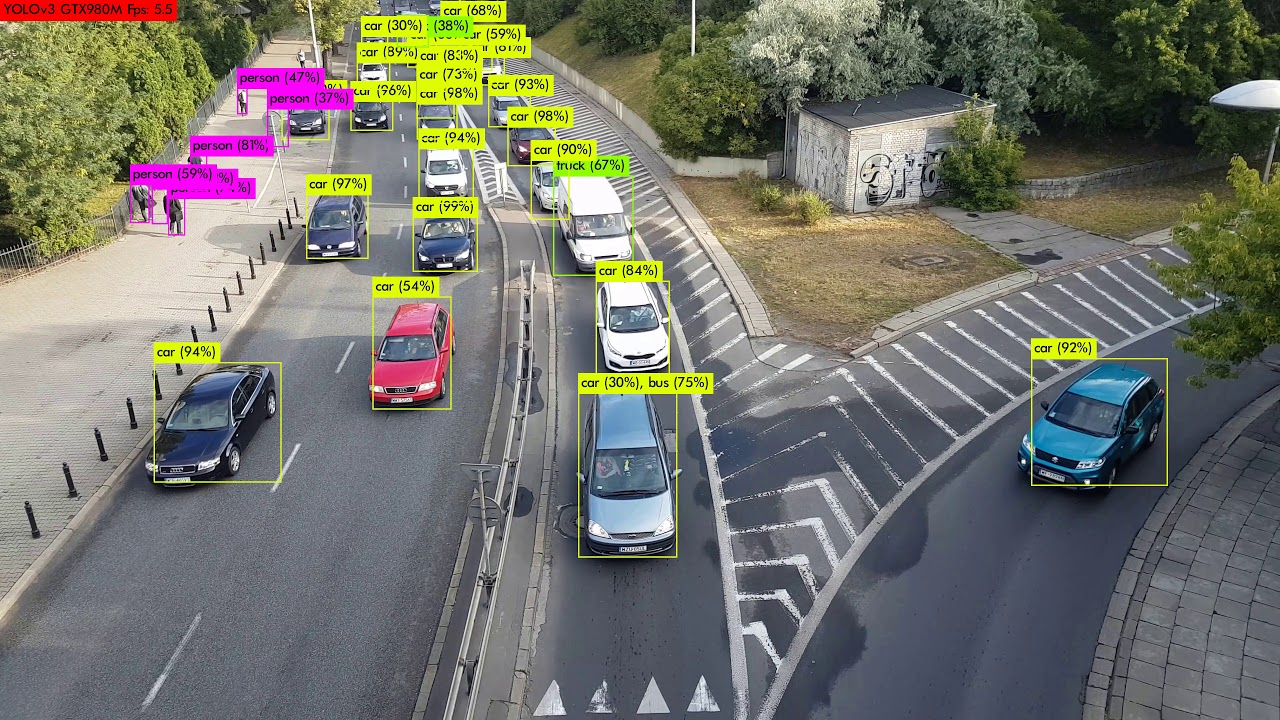
\includegraphics[width=10cm]{figs/yolo}
	\end{figure}
	\note[item]{Visión artificial con aplicaciones como la detección de objetos. Para ello se utilizan técnicas de Deep Learning que explicaremos a continuación.}
\end{frame}

\begin{frame}
	\frametitle{\textit{Deep Learning}}
	\begin{outline}
		\1 \textcolor{red}{Neocognitrón} (1979): Red neuronal con 5 o 6 capas para \textcolor{red}{reconocer caracteres japoneses}.
	\end{outline}
	\begin{figure}
		\centering
		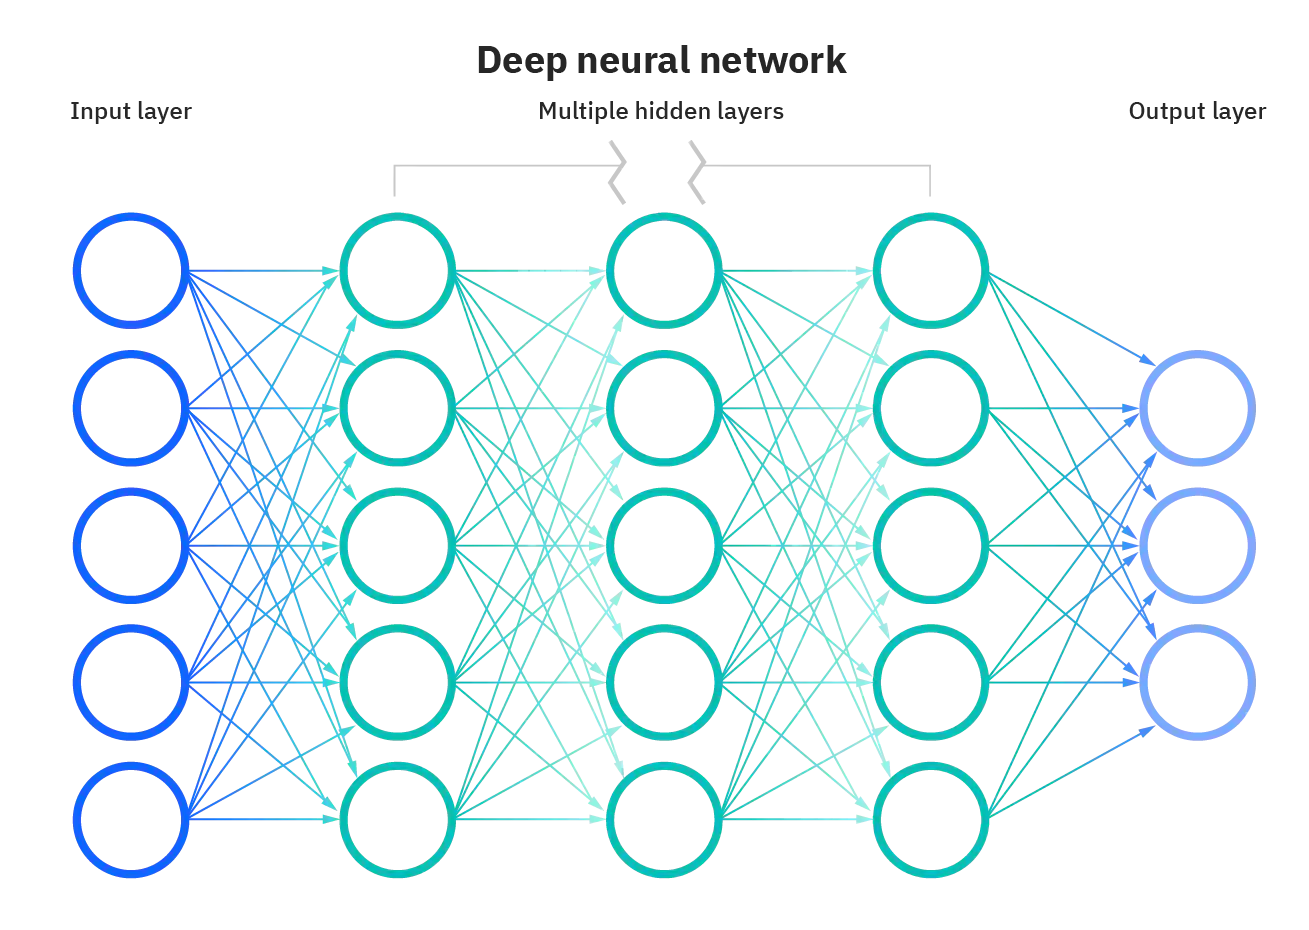
\includegraphics[width=6cm]{figs/neuralnetwork}
	\end{figure}
	\note[item]{Deep Learning No existe límite claro para definir red neuronal Deep Learning.}
\end{frame}

\subsection{Contexto específico}
\begin{frame}
	\frametitle{Vehículos autónomos}
	\begin{figure}
		\centering
		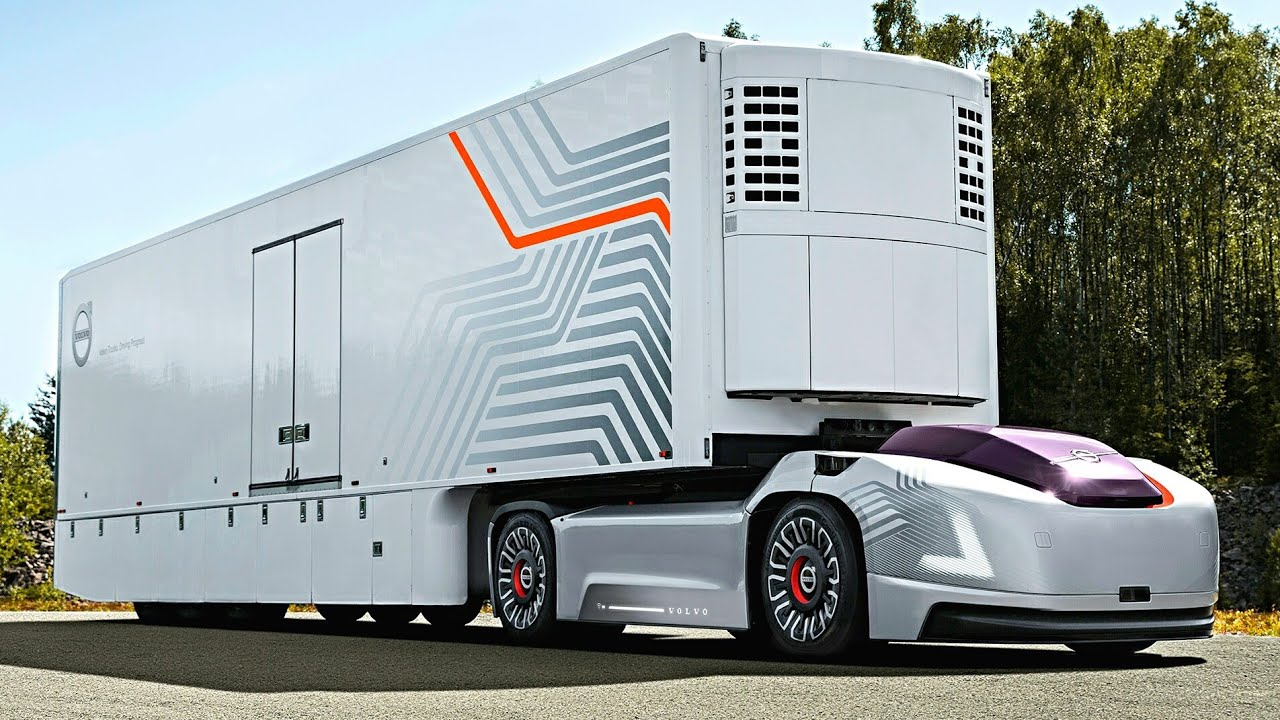
\includegraphics[width=10cm]{figs/volvovera}
	\end{figure}
	\note[item]{Nivel de autonomía 5.}
\end{frame}

\begin{frame}
	\begin{outline}
		\1 Sucesores de los \textcolor{red}{AGVs}.
	\end{outline}
	\frametitle{\textit{AMRs}}
	\begin{figure}
		\centering
		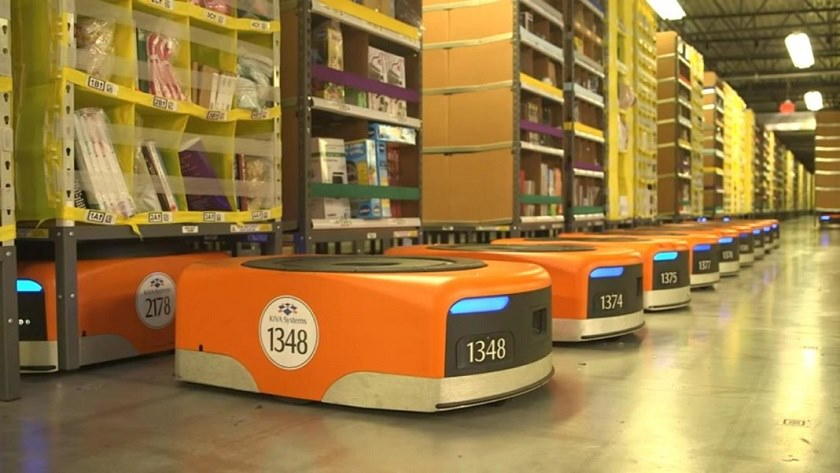
\includegraphics[width=8cm]{figs/kivasystems}
	\end{figure}
	\note[item]{Kiva Systems.}
\end{frame}

%%%%%%%%%%%%%%%%%%%%%%%%%%%%%%%%%%%%%%%%%%%%%%%%%%%%%%%%% Capítulo 2 %%%%%%%%%%%%%%%%%%%%%%%%%%%%%%%%%%%%%%%%%%%%%%%%%%%%%%%%%%%%%%%% 

\section*{}
\begin{frame}{}
	\centering \Huge
	\emph{Objetivos}
	\note[item]{Objetivos.}
\end{frame}

\section{Objetivos}
\subsection{Descripción del problema}
\begin{frame}
	\frametitle{Descripción del problema}
	\begin{outline}
		\1 Desarrollar un \textcolor{red}{coche autónomo }capaz de circular por un \textcolor{red}{circuito} en un entorno dinámico, interactuando con objetos propios de
		una ciudad en dos entornos
		distintos:
		\2 Entorno \textcolor{red}{simulado} con \textcolor{red}{\textit{Gazebo}}.
		\2 Entorno \textcolor{red}{real} usando un robot con \textcolor{red}{\textit{Jetson Nano}}.
		\1 En ambos entornos se han de cumplir dos subobjetivos:
		\2 Seguimiento de \textcolor{red}{carril}
		\2 Detección de \textcolor{red}{objetos}
	\end{outline}
	\note[item]{Descripción.}
\end{frame}

\subsection{Requisitos}
\begin{frame}
	\frametitle{Requisitos}
	\begin{itemize}
		\item El sistema operativo utilizado será \textcolor{red}{\textit{GNU/Linux}}, concretamente la distribución \textcolor{red}{\textit{Ubuntu 18.04 LTS}}.
		\item El entorno simulado requerirá la presencia de una tarjeta gráfica dedicada: \textcolor{red}{\textit{NVIDIA}} y \textcolor{red}{\textit{CUDA}}.
		\item El entorno real requerirá un robot con la placa de desarrollo \textcolor{red}{\textit{NVIDIA Jetson Nano}}, ya que esta es una de las placas con
		      \textcolor{red}{\textit{GPU}} más económicas.
		\item El lenguaje de programación utilizado será \textcolor{red}{\textit{Python}}.
	\end{itemize}
	\note[item]{Requisitos.}
\end{frame}

%%%%%%%%%%%%%%%%%%%%%%%%%%%%%%%%%%%%%%%%%%%%%%%%%%%%%%%% Capítulo 3 %%%%%%%%%%%%%%%%%%%%%%%%%%%%%%%%%%%%%%%%%%%%%%%%%%%%%%%%%%%%%%% 

\section*{}
\begin{frame}{}
	\centering \Huge
	\emph{Plataforma de desarrollo}
	\note[item]{Plataforma de desarrollo.}
\end{frame}

\section{Plataforma de desarrollo}
\subsection{Hardware}
\begin{frame}
	\frametitle{NVIDIA Jetson Nano}
	\begin{outline}
		\1 Placa de desarrollo de \textcolor{red}{bajo coste} con \textcolor{red}{GPU} dedicada.
		\1 Arquitectura \textcolor{red}{\textit{Aarch64}}, soporte para \textcolor{red}{\textit{GNU/Linux}} y puertos \textcolor{red}{\textit{GPIO}}.
	\end{outline}
	\begin{figure}
		\centering
		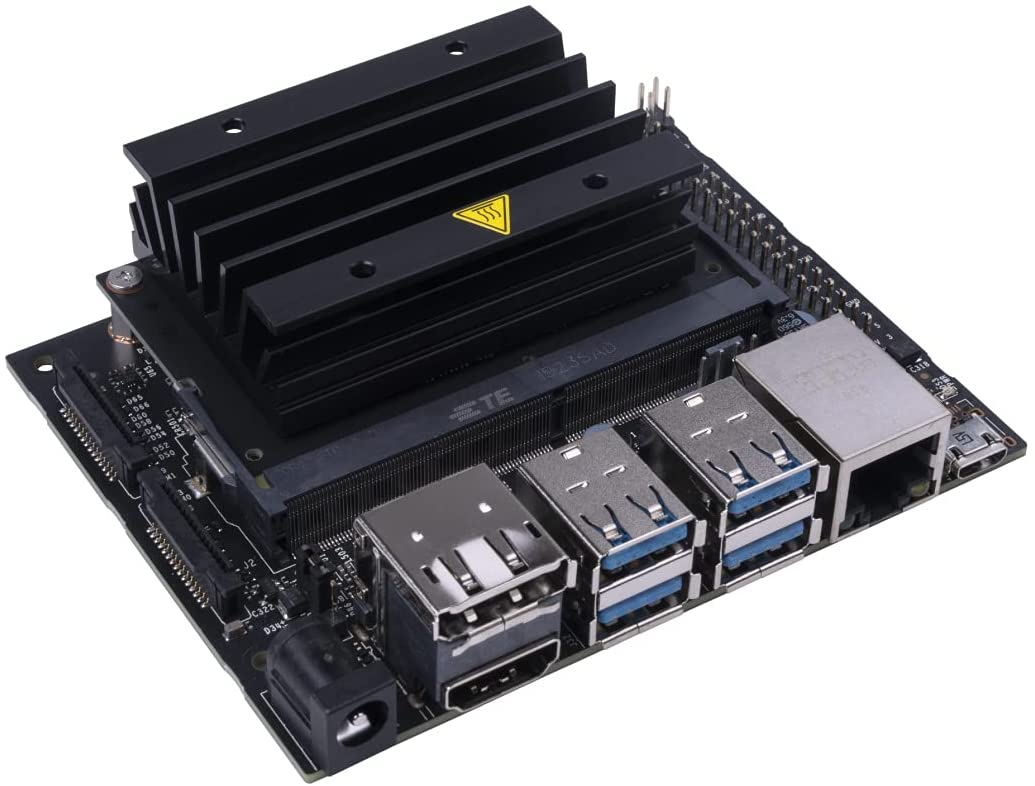
\includegraphics[width=6cm]{figs/jetsonnano}
	\end{figure}
	\note[item]{NVIDIA Jetson Nano.}
\end{frame}
\begin{frame}
	\frametitle{Componentes}
	\begin{figure}
		\centering
		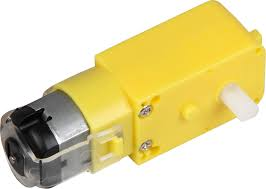
\includegraphics[width=3cm]{figs/motorTT}
		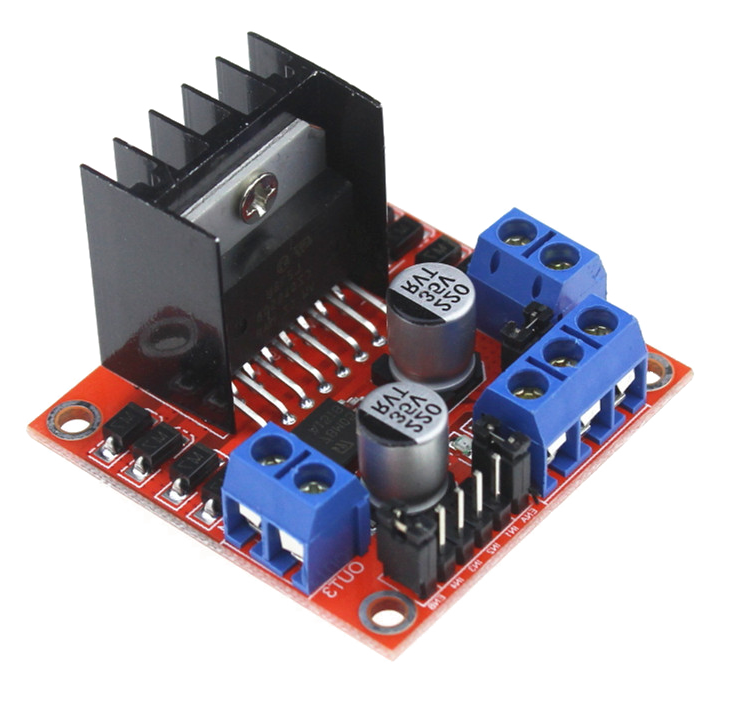
\includegraphics[width=3cm]{figs/l298n}
		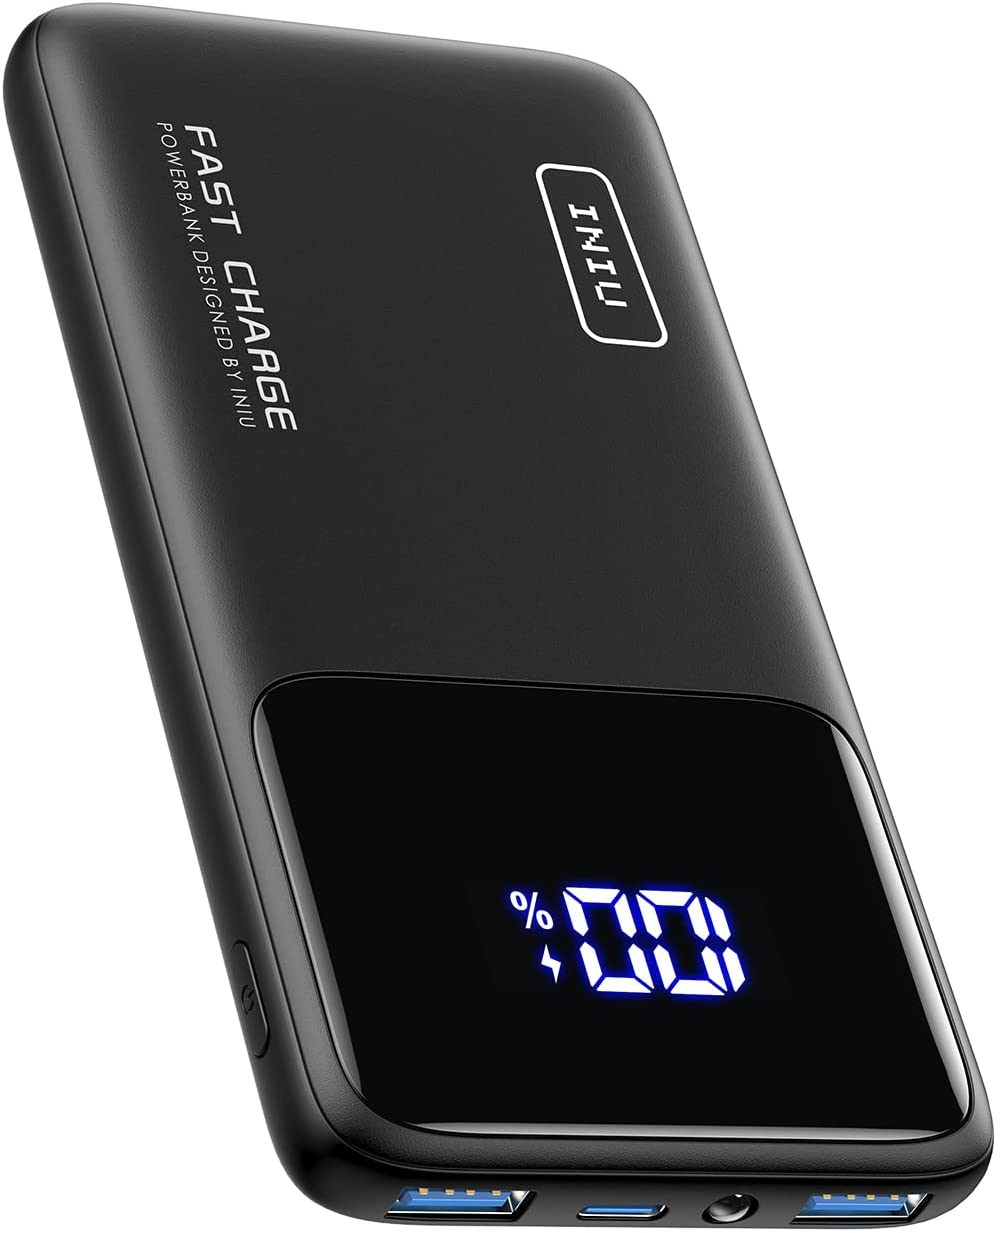
\includegraphics[width=2.5cm]{figs/battery2}
		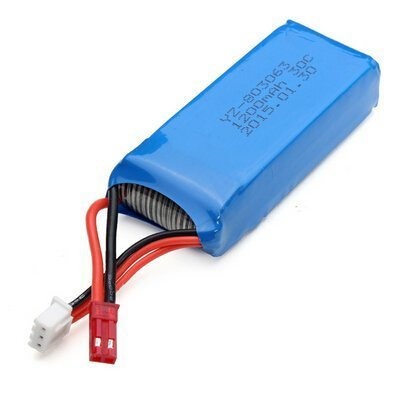
\includegraphics[width=3cm]{figs/tarantula}
		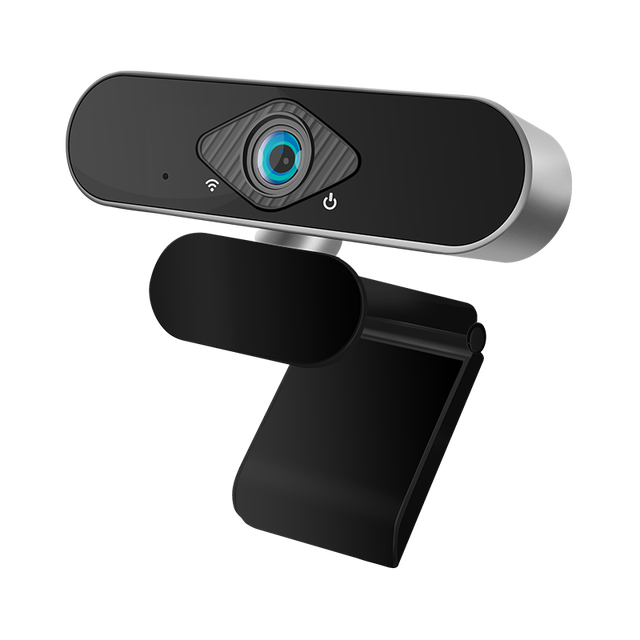
\includegraphics[width=3cm]{figs/camera}
		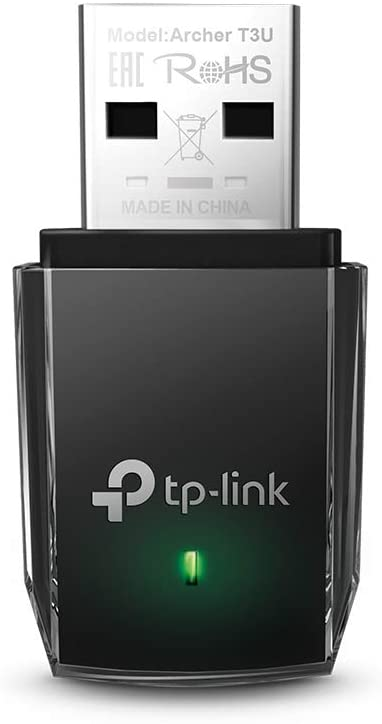
\includegraphics[width=1.5cm]{figs/tplink}
		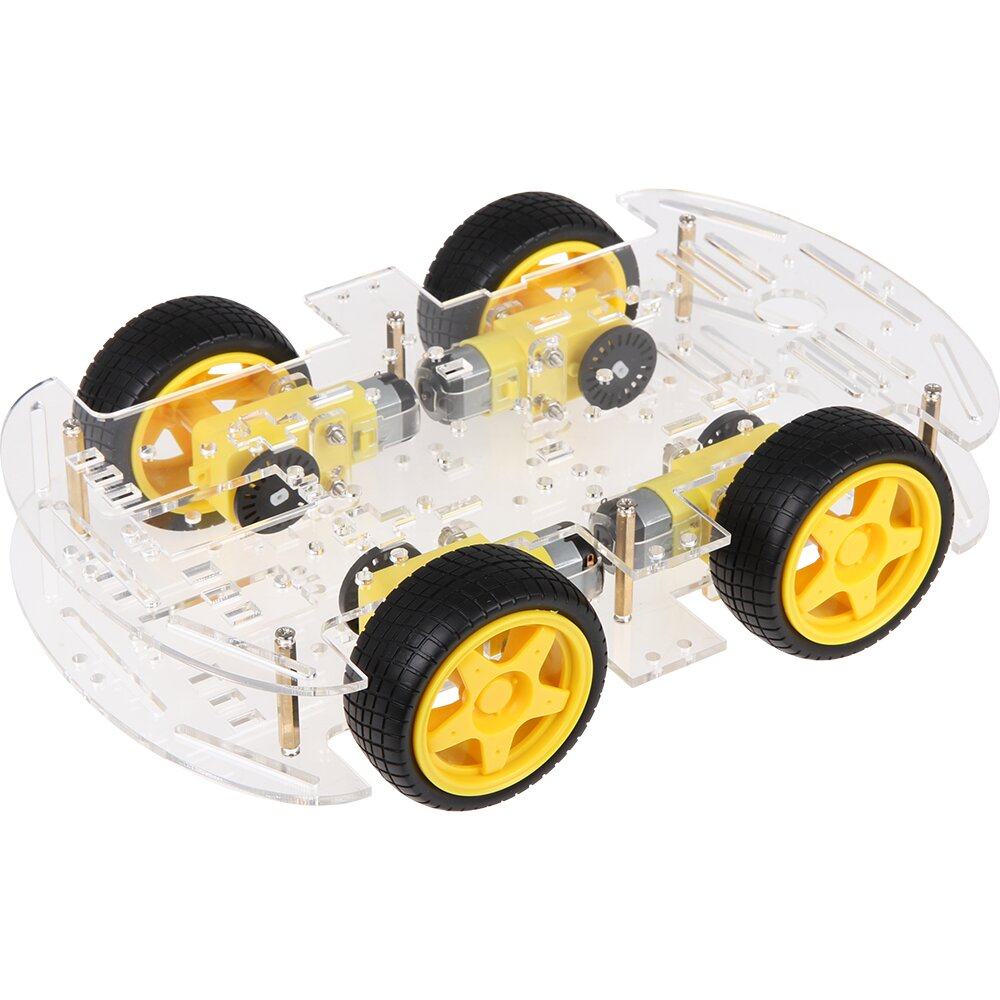
\includegraphics[width=3.5cm]{figs/chasis}
	\end{figure}
	\note[item]{Componentes.}
	\note[item]{Motores de bajo coste sin odometría.}
	\note[item]{Controlador de motores. Limitaciones motores a pares.}
	\note[item]{Batería 10000mAh para alimentar Jetson Nano.}
	\note[item]{Batería 7.4V para alimentar motores.}
	\note[item]{Cámara USB como sensor principal.}
	\note[item]{Adaptador Wi-Fi para conexión mediante SSH con el robot.}
	\note[item]{Chasis muy usado en proyectos relacionados con Arduino.}
\end{frame}

\subsection{Software}
\begin{frame}
	\frametitle{Software}
	\begin{figure}
		\centering
		
\includegraphics[width=2cm]{figs/pythonlogo}\hspace{0.5cm}
		
\includegraphics[width=2cm]{figs/freecadlogo}\hspace{0.3cm}
		
\includegraphics[width=2.3cm]{figs/blenderlogo}\hspace{0.5cm}
		
\includegraphics[width=1.7cm]{figs/gazebologo}\\
		\vspace{1cm}
\includegraphics[width=4.3cm]{figs/roslogo}\hspace{0.5cm}
		
\includegraphics[width=4cm]{figs/pyqtlogo}
	\end{figure}
	\note[item]{Software.}
	\note[item]{Python.}
	\note[item]{FreeCAD.}
	\note[item]{Blender.}
	\note[item]{Gazebo.}
	\note[item]{ROS.}
	\note[item]{PyQT.}
\end{frame}

\begin{frame}
	\frametitle{Software relacionado con visión}
	\begin{figure}
		\centering
		
\includegraphics[height=2cm]{figs/opencvlogo}\hspace{0.8cm}
		
\includegraphics[height=1.5cm]{figs/yolologo}\hspace{0.6cm}
		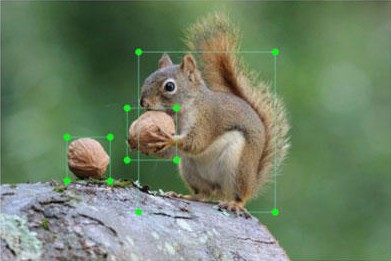
\includegraphics[width=3.3cm]{figs/labelimg}\hspace{0.8cm}\\
		\vspace{1cm}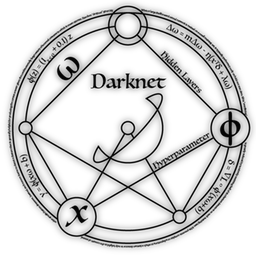
\includegraphics[width=2.8cm]{figs/darknetlogo}\hspace{0.8cm}
		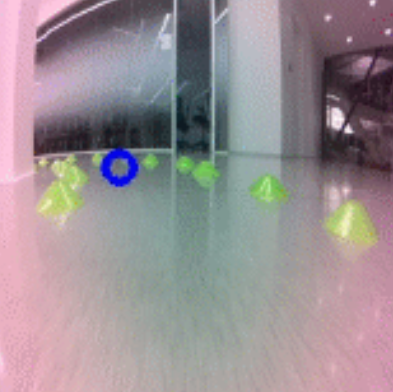
\includegraphics[width=2.8cm]{figs/jetracerframe}
	\end{figure}
	\note[item]{Software relacionado con visión.}
	\note[item]{OpenCV.}
	\note[item]{YOLO.}
	\note[item]{LabelIMG.}
	\note[item]{Darknet.}
	\note[item]{JetRacer.}
\end{frame}

%%%%%%%%%%%%%%%%%%%%%%%%%%%%%%%%%%%%%%%%%%%%%%%%%%%%%%%%% Capítulo 4 %%%%%%%%%%%%%%%%%%%%%%%%%%%%%%%%%%%%%%%%%%%%%%%%%%%%%%%%%% 

\section*{}
\begin{frame}{}
	\centering \Huge
	\emph{Sistema de conducción autónoma}
	\note[item]{Una vez descritos los objetivos y las plataformas utilizadas veamos el desarrollo en sí del proyecto.}
\end{frame}

\section{Sistema de conducción autónoma}
\subsection{Entorno simulado}
\begin{frame}
	\frametitle{Modelo de la ciudad en \textit{Gazebo}}
	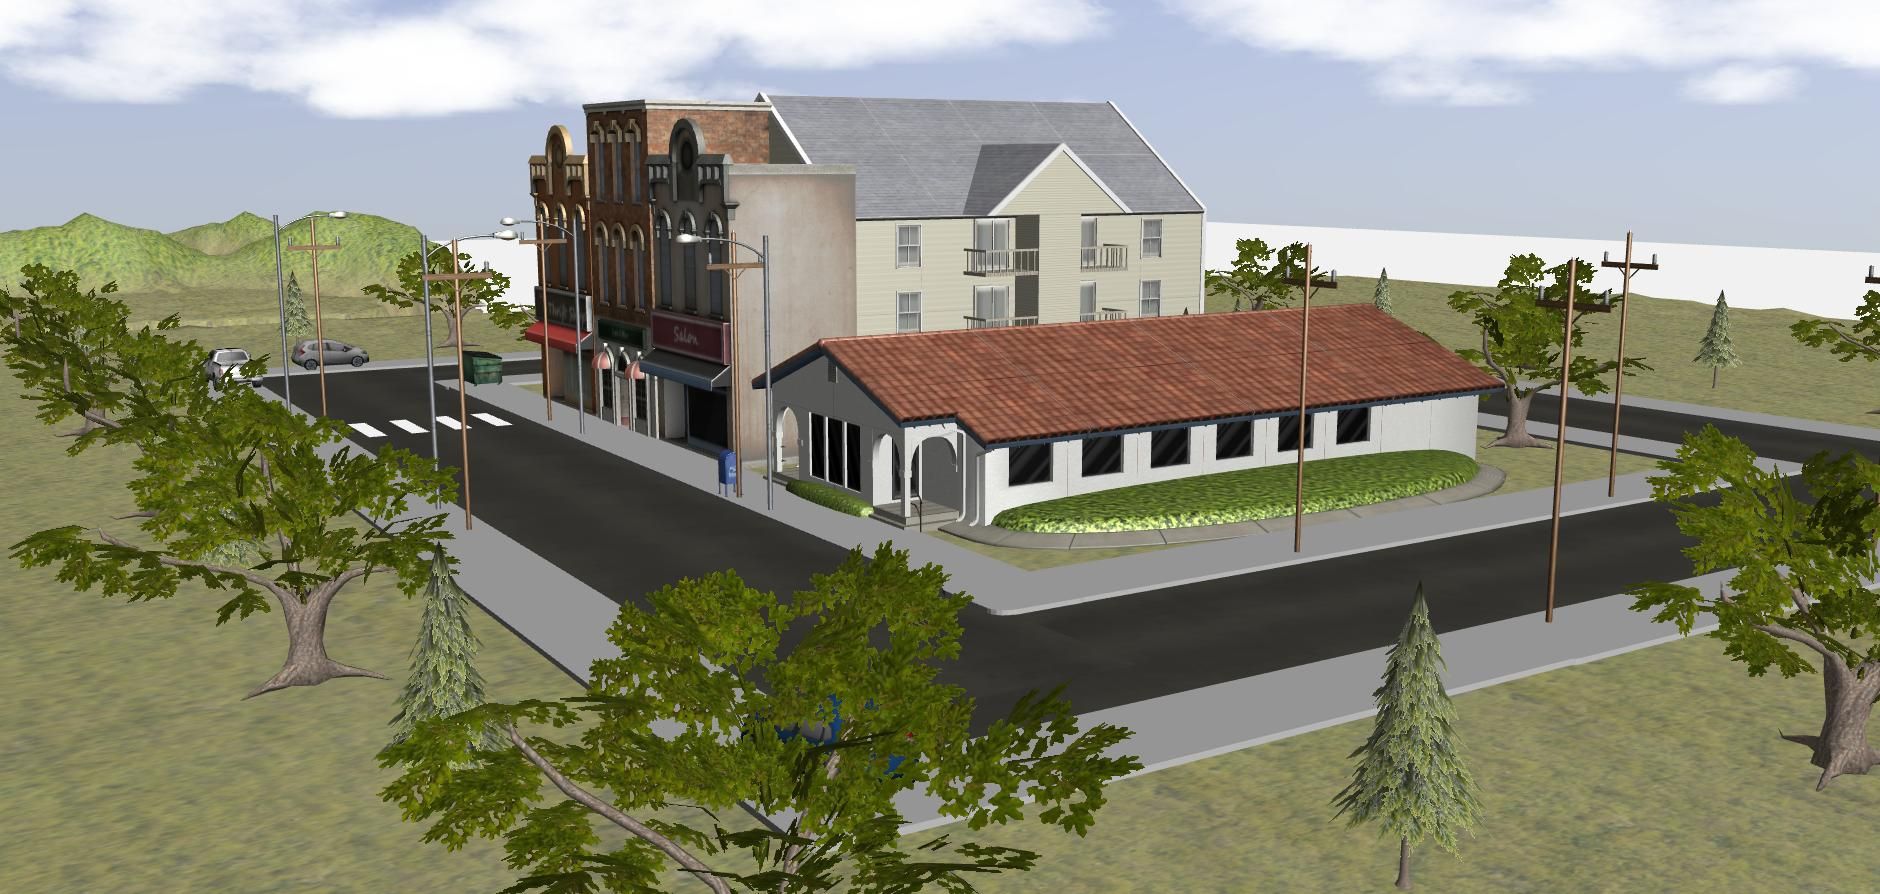
\includegraphics[height=3cm]{figs/smallcity}
	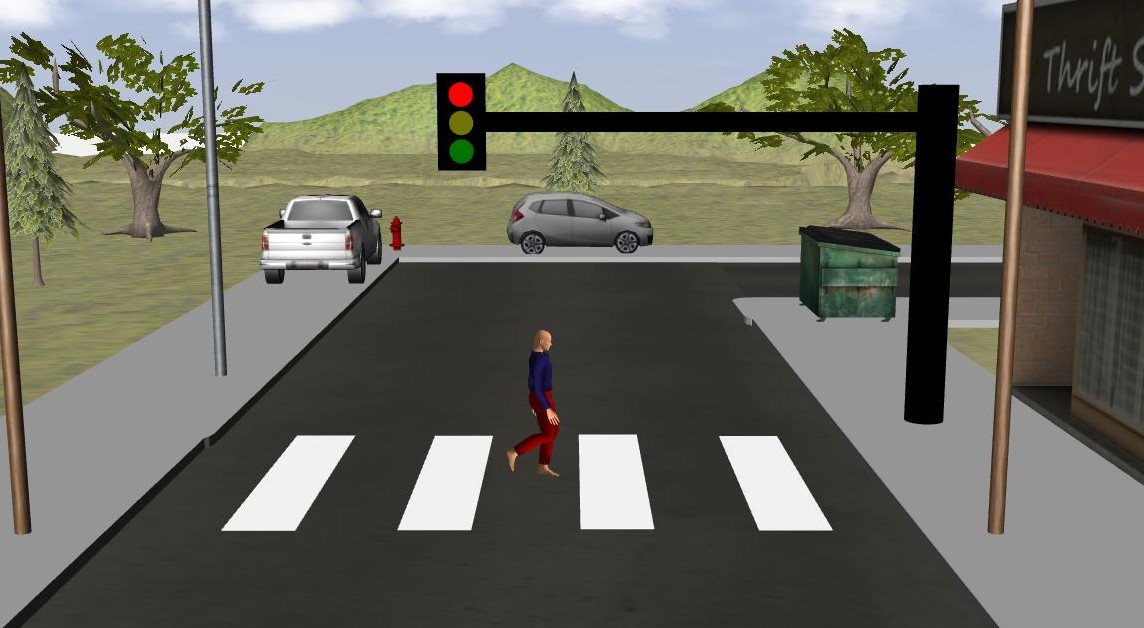
\includegraphics[height=3cm]{figs/trafficlightpedestrian}\vspace{1cm}
	\begin{itemize}
		\item Reproducible en el entorno real
		\item Semáforo y peatón dinámico
	\end{itemize}
	\note[item]{Modelo.}
\end{frame}

\begin{frame}
	\frametitle{Modelo del vehículo en \textit{FreeCAD}}
	\begin{figure}
		\centering
		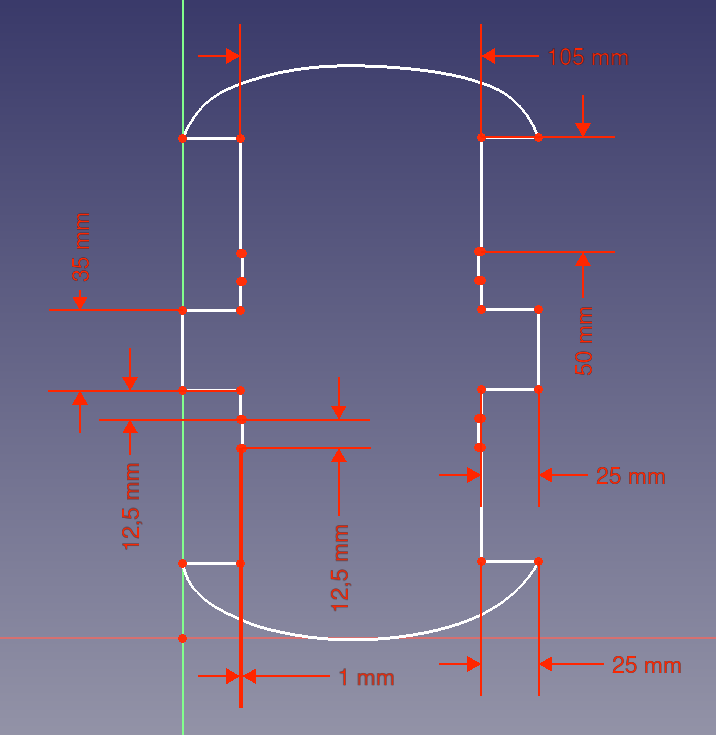
\includegraphics[height=4cm]{figs/sketchFreecad}\hspace{0.1cm}
		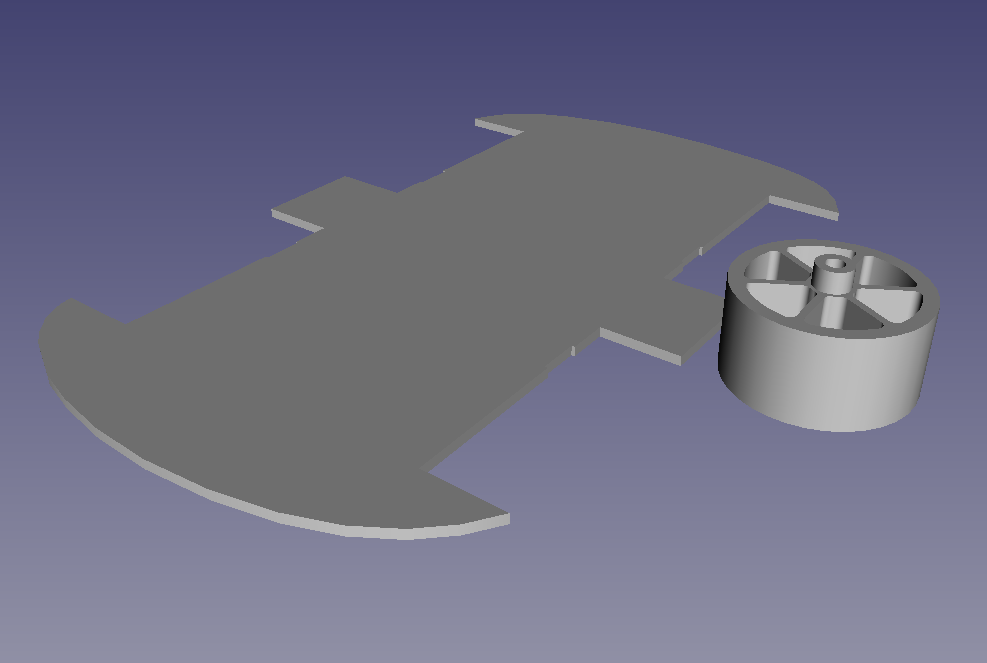
\includegraphics[height=4cm]{figs/freecad}
	\end{figure}
	\note[item]{Modelo del coche autónomo.}
\end{frame}

\begin{frame}
	\frametitle{Modelo y jerarquía del vehículo en \textit{Blender}}
	\begin{figure}
		\centering
		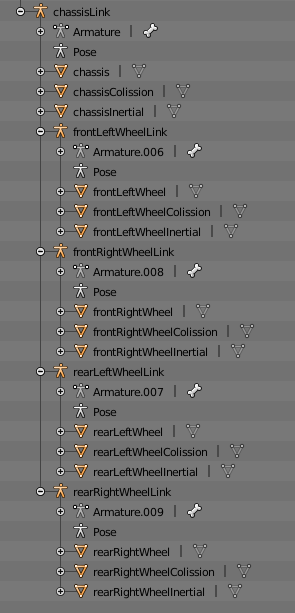
\includegraphics[height=7cm]{figs/phobosDiagram}\hspace{0.1cm}
		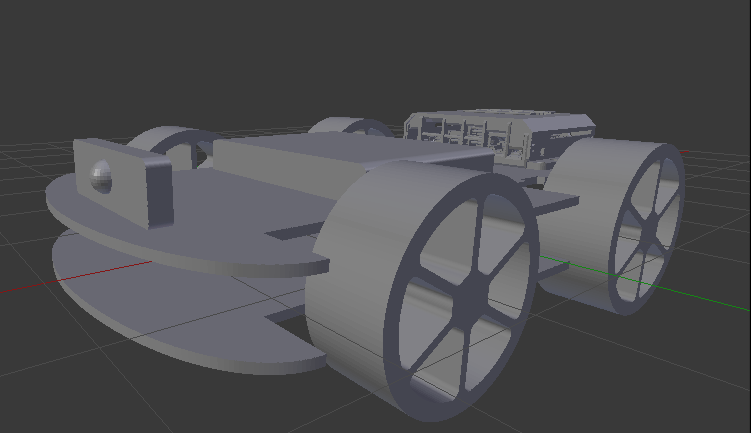
\includegraphics[width=6cm]{figs/blenderModel}
	\end{figure}
	\note[item]{Modelo y jerarquía en Blender.}
\end{frame}

\begin{frame}
	\frametitle{Modelo del vehículo en \textit{Gazebo}}
	\begin{figure}
		\centering
		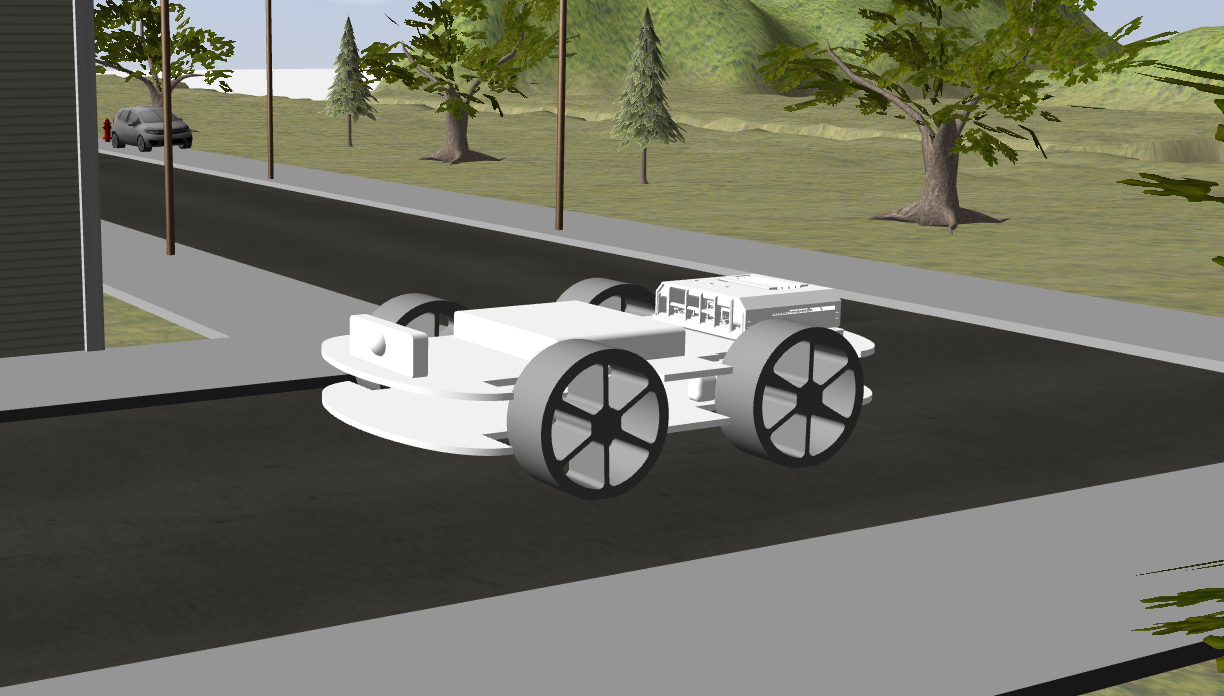
\includegraphics[width=8cm]{figs/modelGazebo}
	\end{figure}
	\begin{outline}
		\1 \textcolor{red}{\textit{Plugins}} para movimiento y cámara conectados con \textcolor{red}{\textit{ROS}}
	\end{outline}
	\note[item]{Modelo del vehículo en Gazebo.}
\end{frame}

\begin{frame}
	\frametitle{Diagrama de clases}
	\begin{figure}
		\centering
		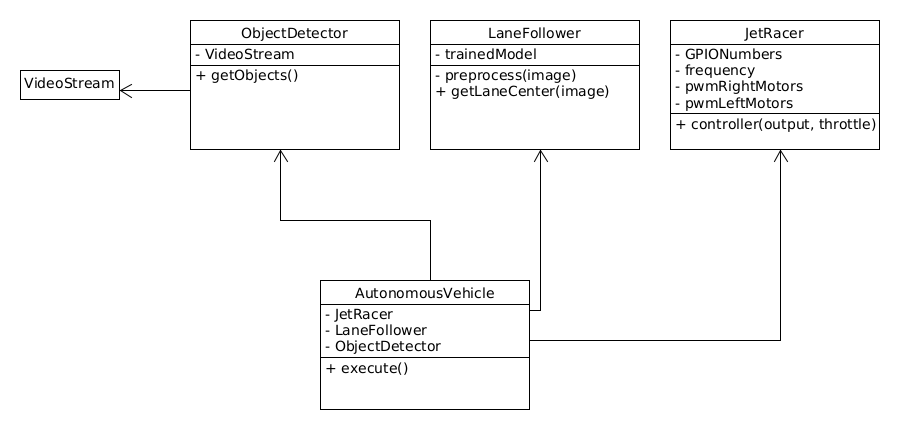
\includegraphics[width=10cm]{figs/diagram6}
	\end{figure}
	\note[item]{Diagrama de clases.}
\end{frame}

\begin{frame}
	\frametitle{Seguimiento de carril}
	\begin{figure}
		\centering
		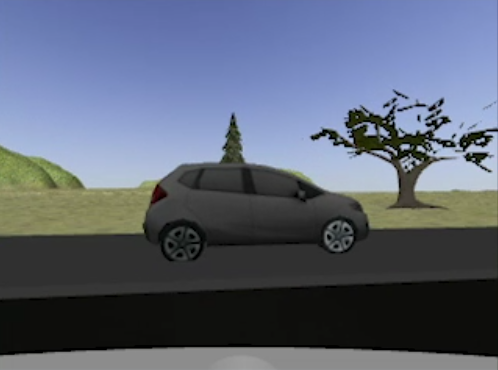
\includegraphics[width=6cm]{figs/trainedDifficult}
	\end{figure}
	\begin{outline}
		\1 Red \textcolor{red}{\textit{ResNet-18}} preentrenada: convolucional de \textcolor{red}{18} capas con \textcolor{red}{bloques residuales}.
		\1 \textit{Notebook} de \textcolor{red}{\textit{Jupyter}}.
		\1 Guardado de cada imagen: \textcolor{red}{\textit{x\_y\_identificador\_unico.jpg}}.
		\1 Dataset con situaciones \textcolor{red}{difíciles}.
	\end{outline}
	\note[item]{PyTorch.}
\end{frame}

\begin{frame}
	\frametitle{Entrenamiento red seguimiento de carril}
	\begin{figure}
		\centering
		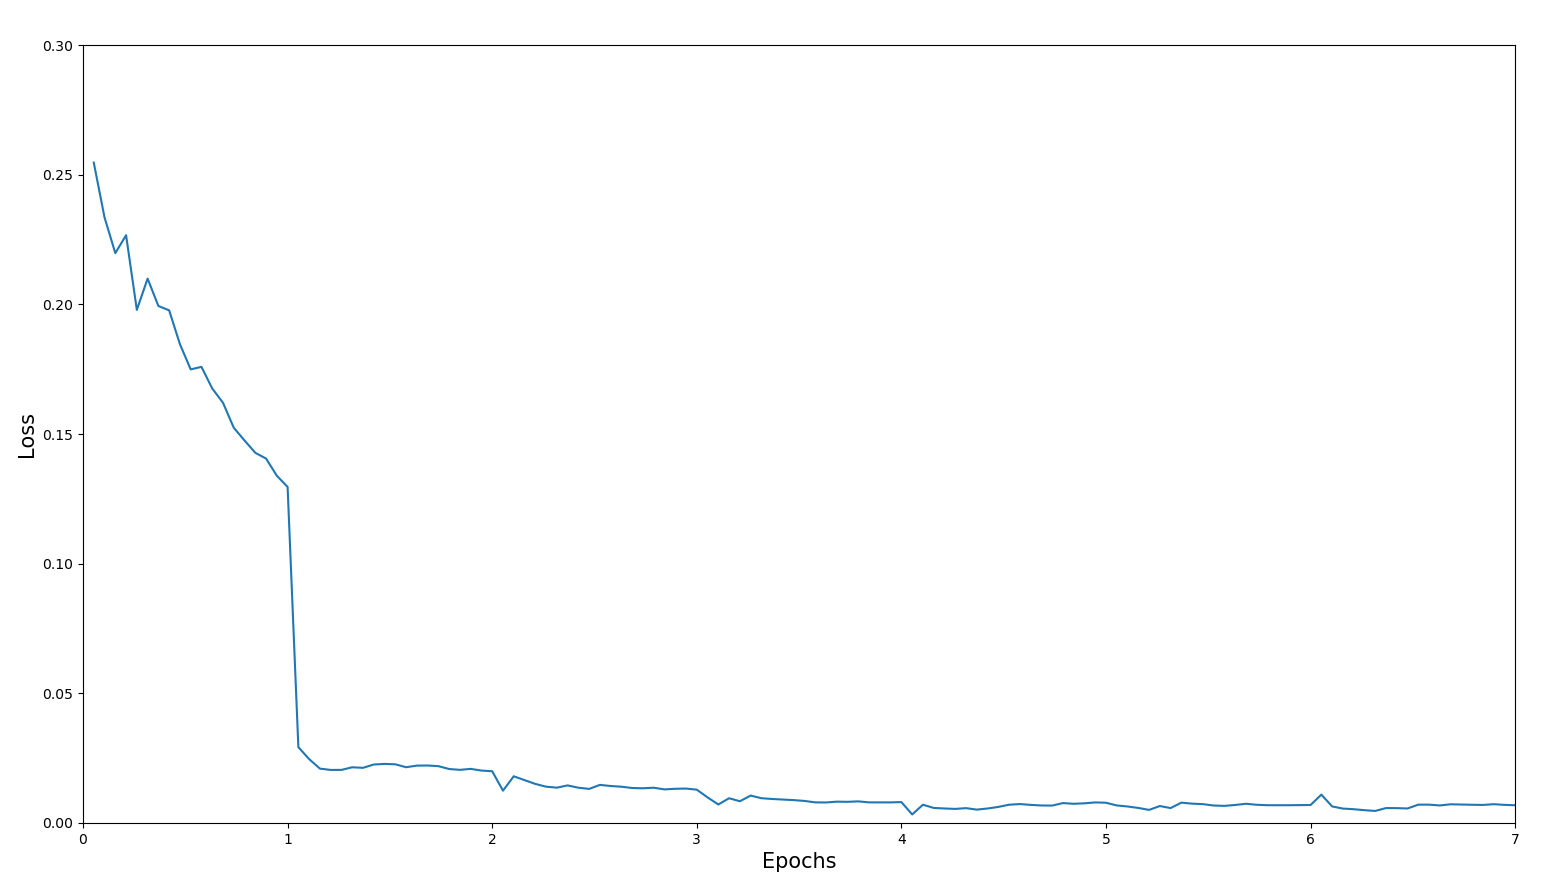
\includegraphics[width=10cm]{figs/simgraphepoch}
	\end{figure}
	\begin{outline}
		\1 En cada \textcolor{red}{\textit{epoch}} se calcula el error cuadrático medio \textcolor{red}{(\textit{loss})}.
		\1 \textcolor{red}{Propagación hacia atrás} de los errores desde la capa de salida hasta la primera capa.
		\1 Error disminuye hasta \textcolor{red}{0.0068}.
	\end{outline}
	\note[item]{Entrenamiento red seguimiento de carrill.}
\end{frame}

\begin{frame}
	\frametitle{Salida red seguimiento de carril}
	\begin{figure}
		\centering
		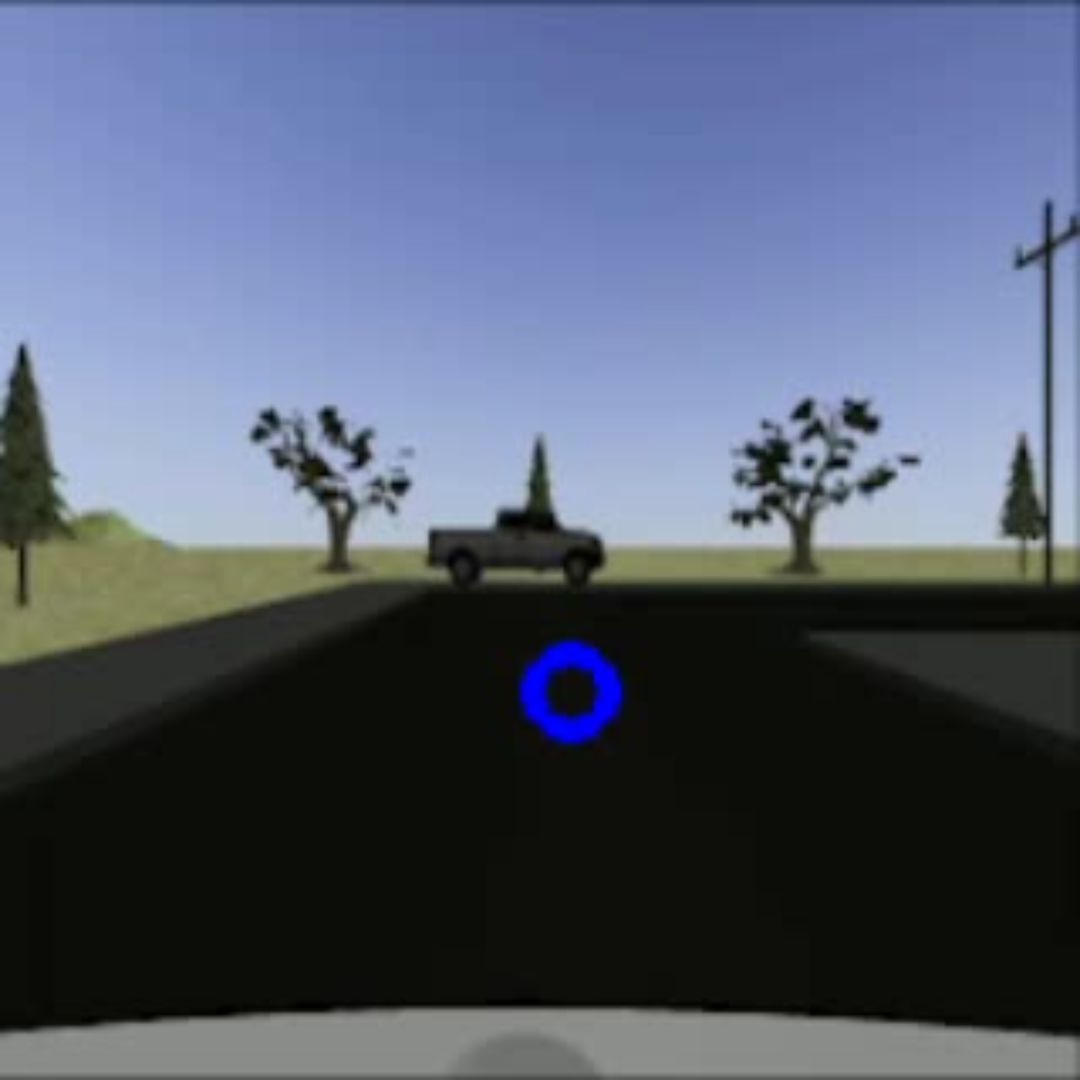
\includegraphics[width=5cm]{figs/outputNNsim}
	\end{figure}
	\begin{outline}
		\1 \textcolor{red}{224} píxeles.
		\1 Entorno experimental: \textcolor{red}{autómata}.
	\end{outline}
	\note[item]{Entrenamiento red seguimiento de carril.}
\end{frame}

\begin{frame}
	\frametitle{Detección de objetos}
	\begin{figure}
		\centering
		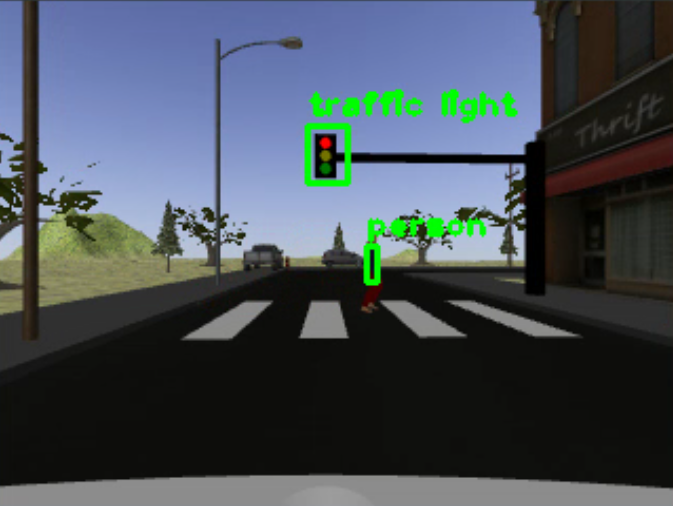
\includegraphics[width=5cm]{figs/darknetSimulator}
	\end{figure}
	\begin{outline}
		\1 \textcolor{red}{\textit{YOLO V3 Tiny}}.
		\1 Objetos muy \textcolor{red}{\textit{genéricos}}: alta probabilidad de detección.
		\1 \textcolor{red}{\textit{Bounding Box}}: clase y probabilidad.
	\end{outline}
	\note[item]{Detección de objetos.}
\end{frame}

\begin{frame}
	\frametitle{Detección de semáforo}
	\begin{figure}
		\centering
		
\includegraphics[width=2cm, height=4cm]{figs/cropped}\hspace{2cm}
\includegraphics[width=2cm, height=4cm]{figs/hsv}\hspace{2cm}
\includegraphics[width=2cm,
			height=4cm]{figs/mask}
	\end{figure}
	\note[item]{Detección de semáforo.}
\end{frame}

\begin{frame}
	\frametitle{Ejecución en el simulador}
	\begin{figure}
		\centering
		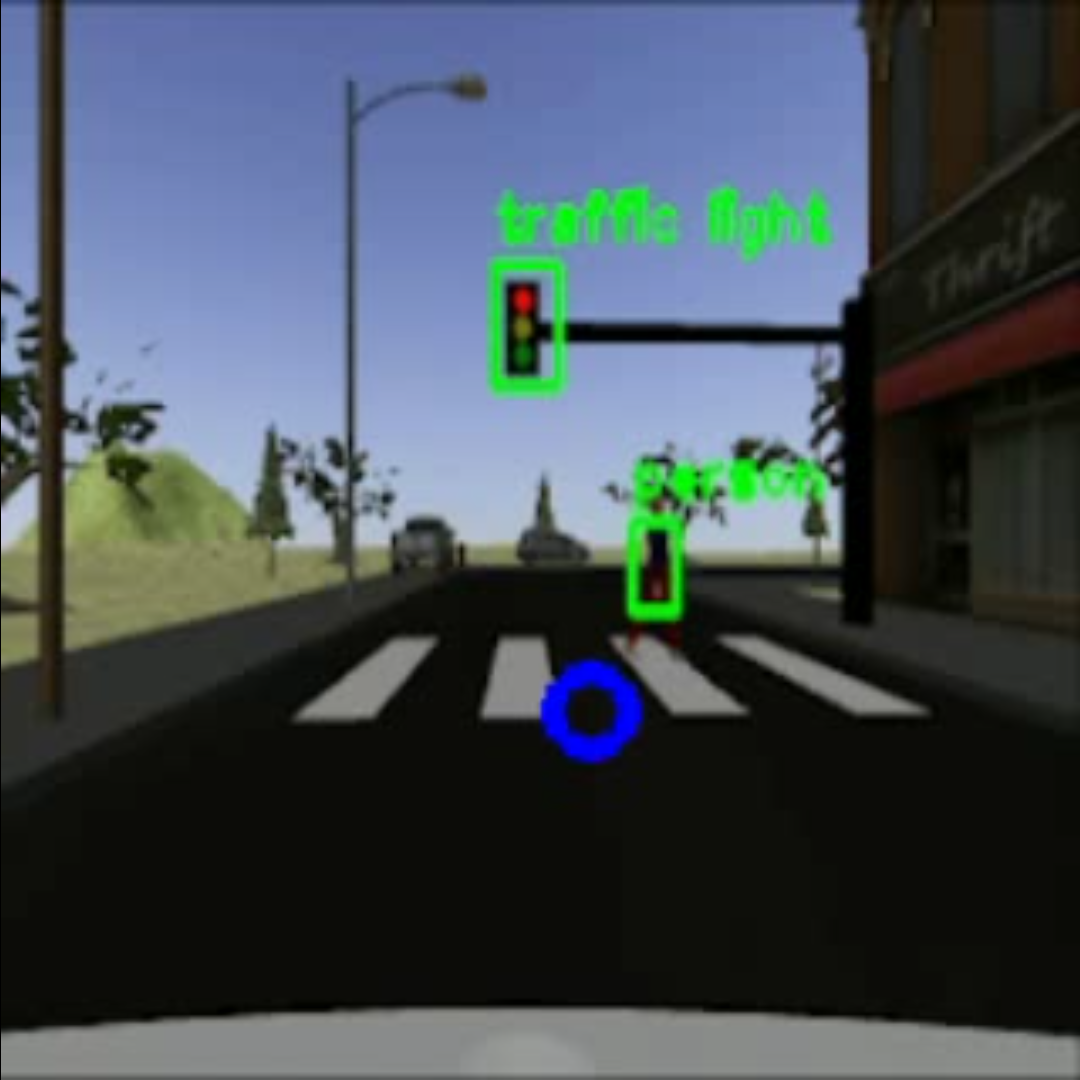
\includegraphics[width=3.25cm]{figs/simRed}\\\vspace{0.5cm}
		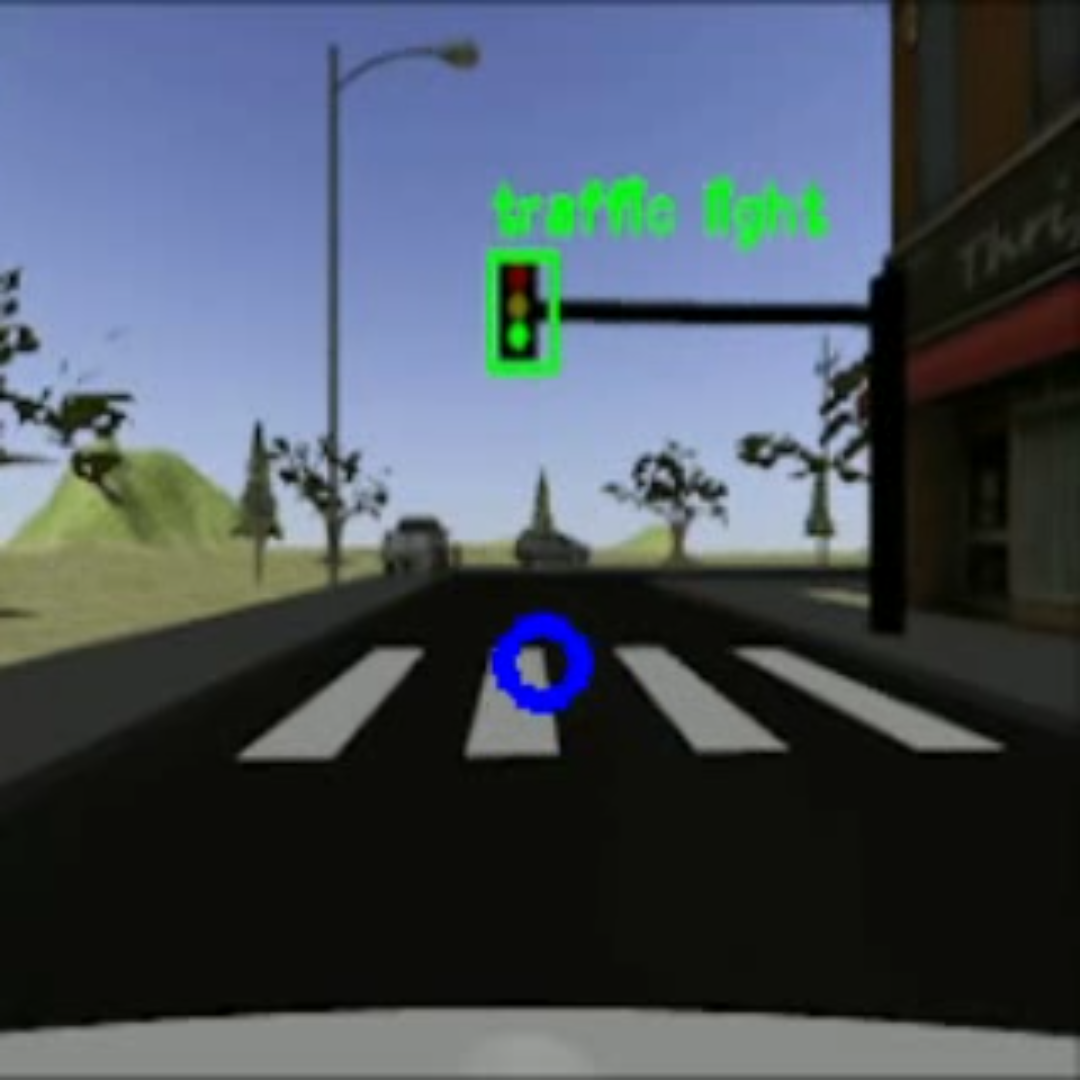
\includegraphics[width=3.25cm]{figs/simGreen}\hspace{1cm}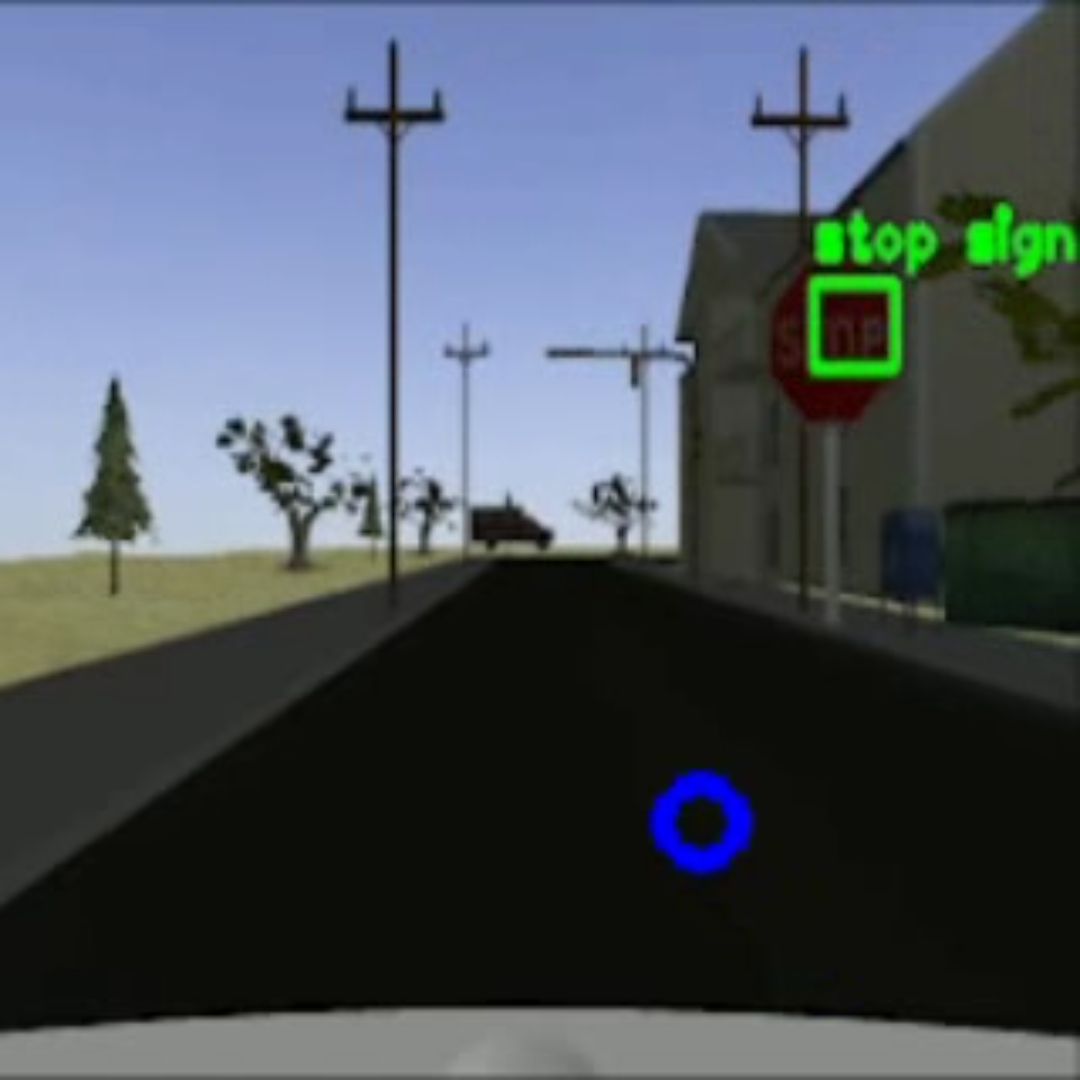
\includegraphics[width=3.25cm]{figs/simStop}
	\end{figure}
	\note[item]{Ejecución en el simulador.}
\end{frame}

\begin{frame}
	\frametitle{Interfaz de usuario}
	\begin{figure}
		\centering
		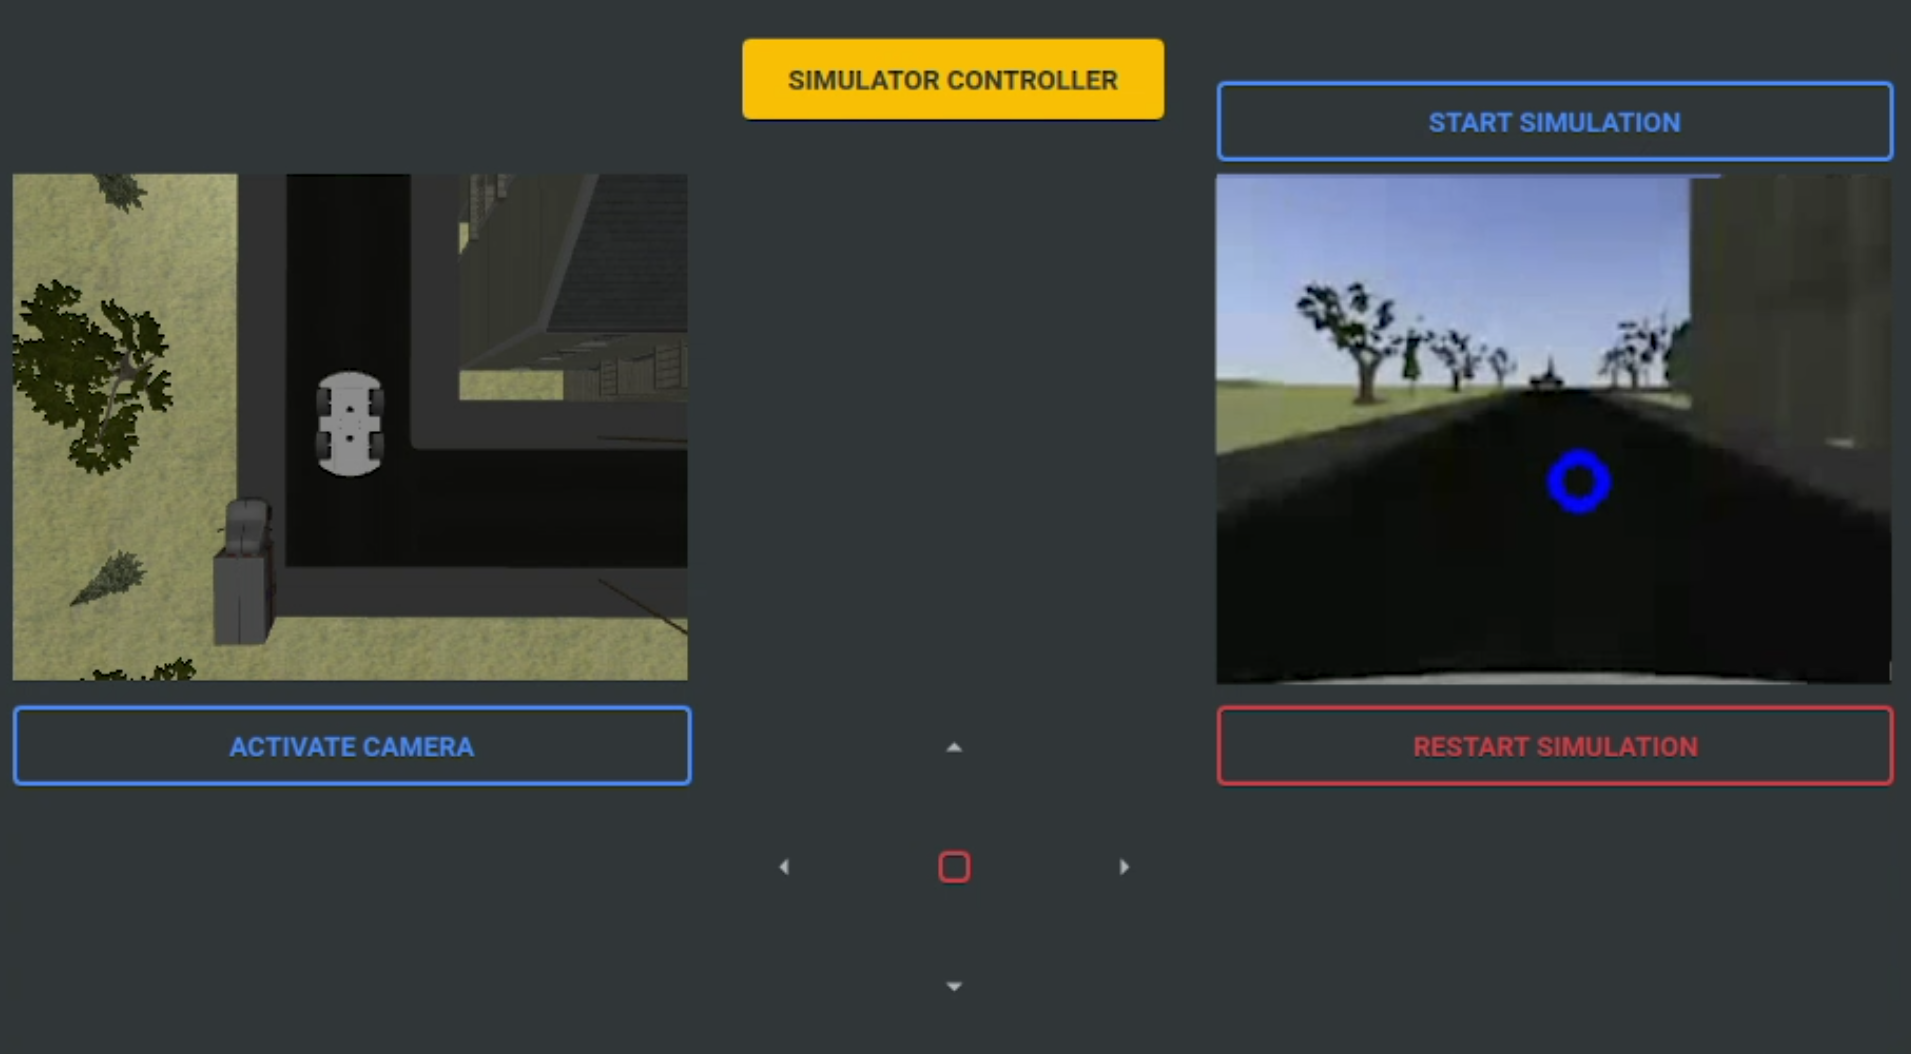
\includegraphics[width=10cm]{figs/GUI}
	\end{figure}
	\note[item]{Interfaz de usuario.}
\end{frame}

\subsection{Entorno real}
\begin{frame}
	\frametitle{Entorno real}
	\begin{figure}
		\centering
		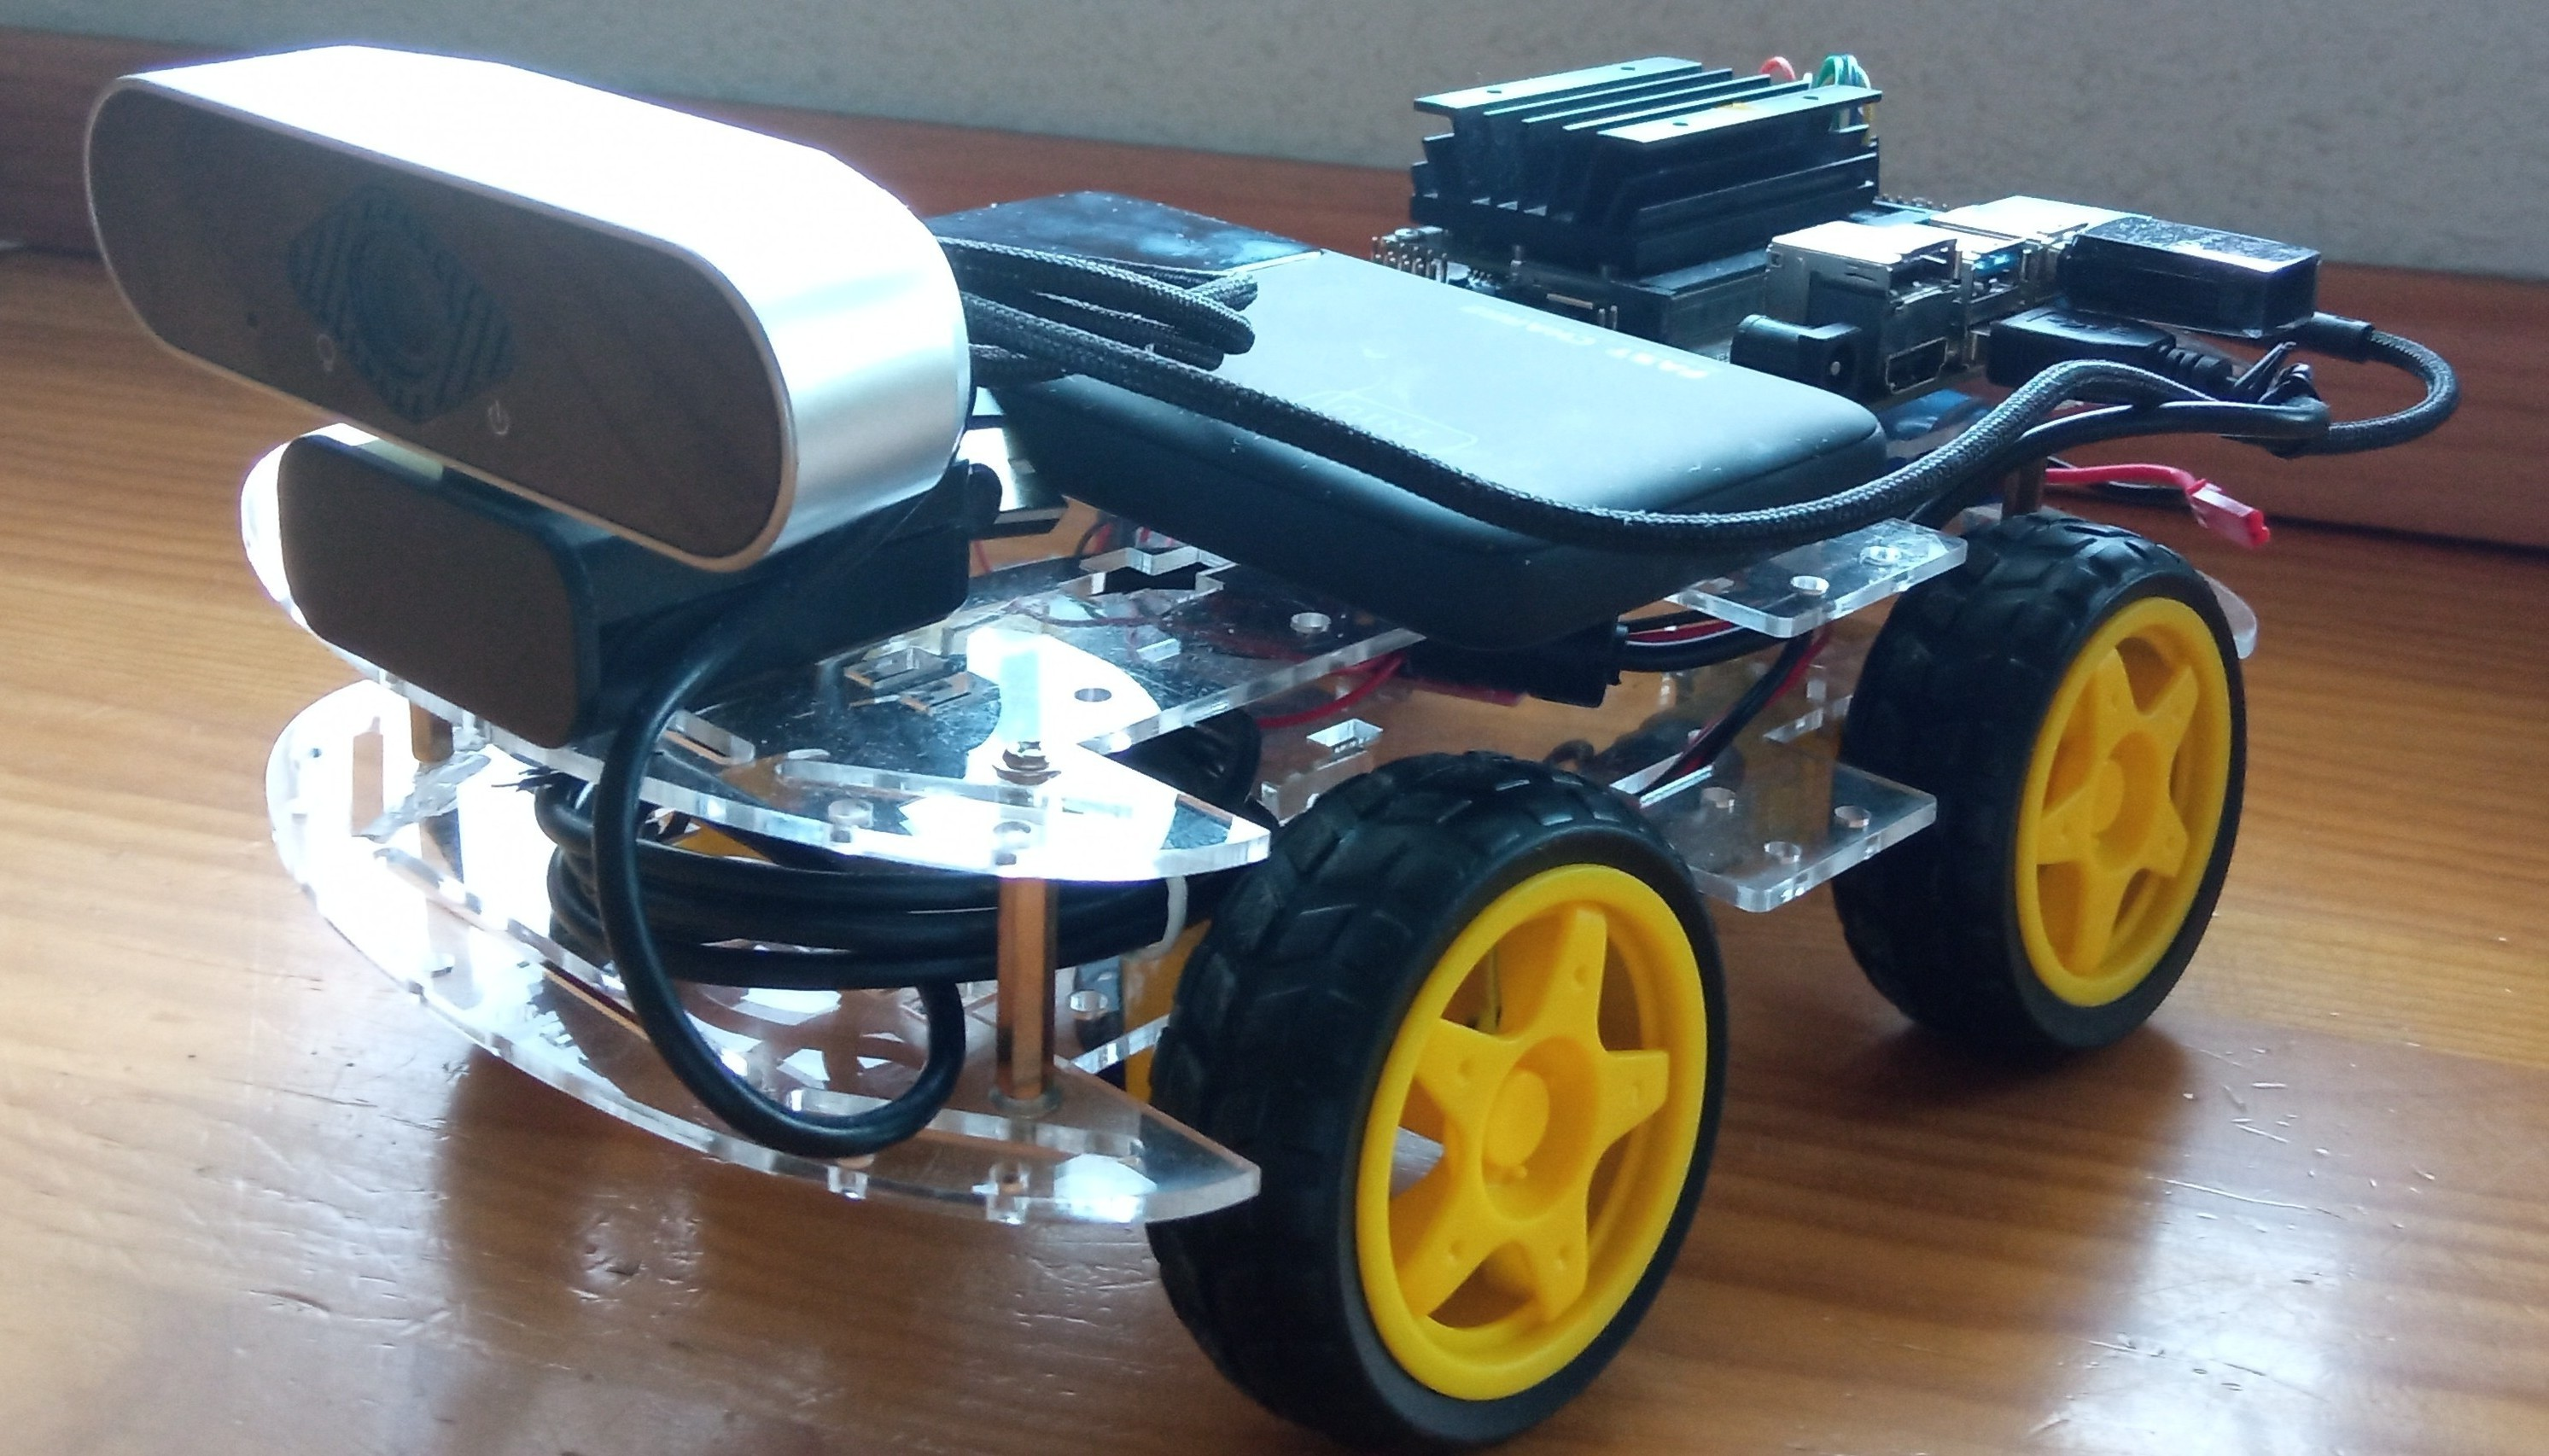
\includegraphics[width=6cm]{figs/robot}\vspace{0.5cm}\\
		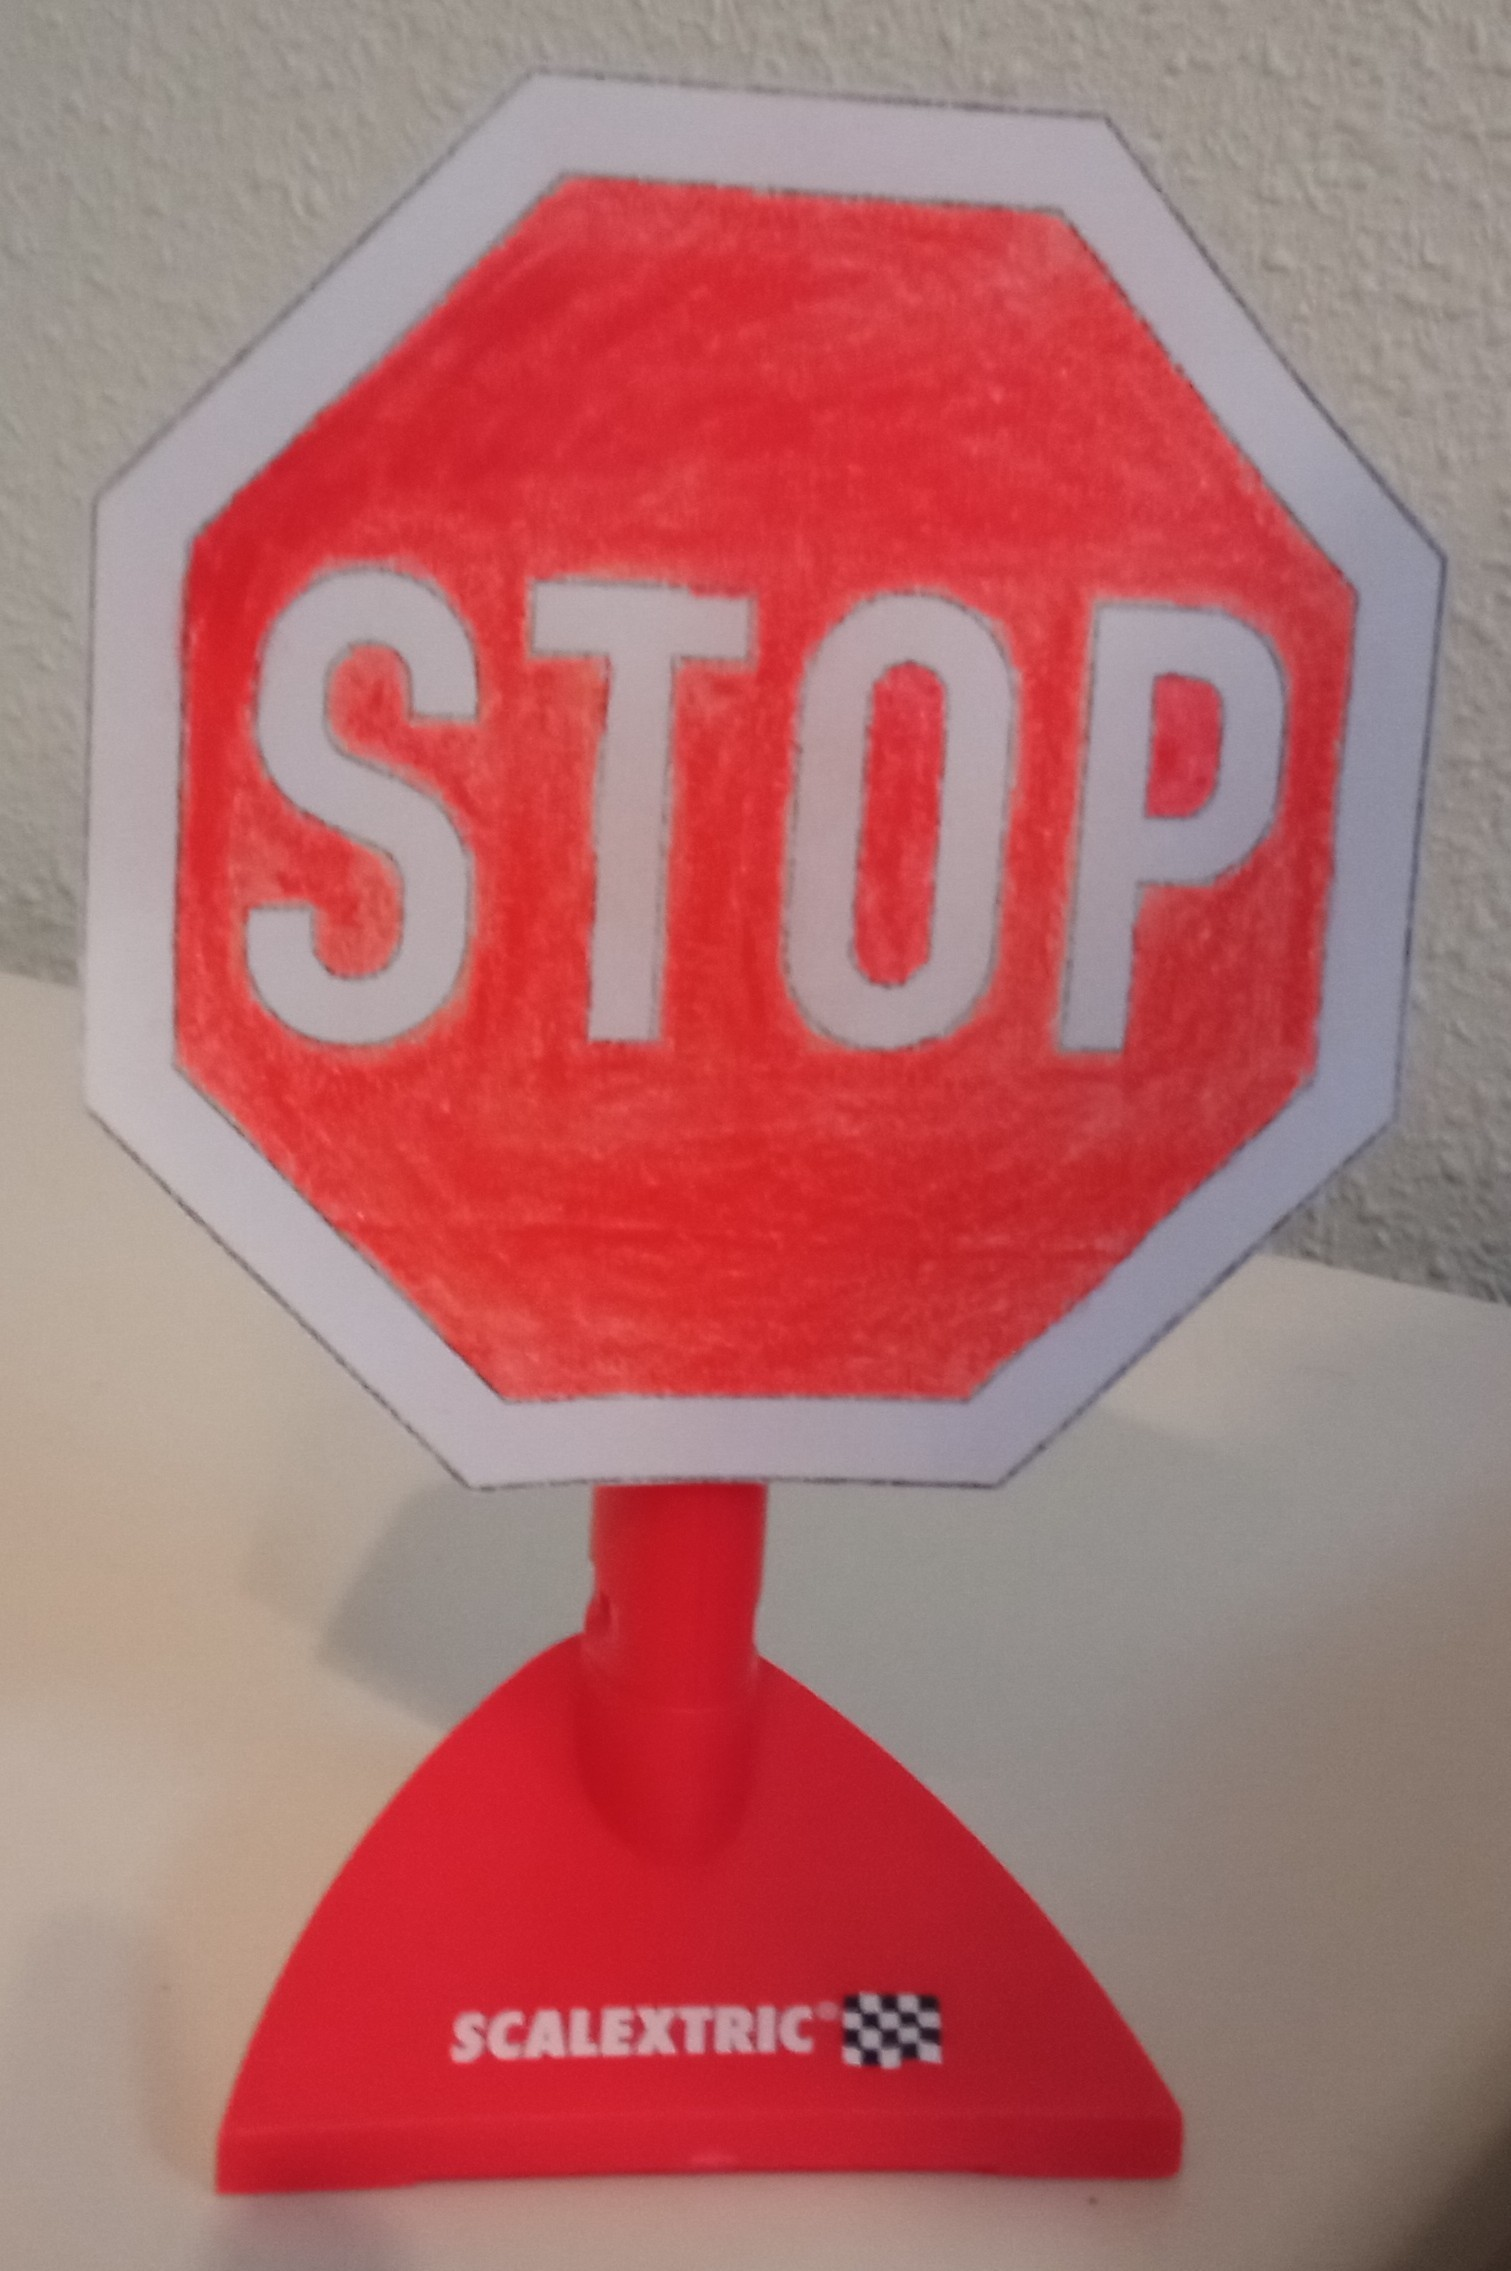
\includegraphics[width=2cm, height=2.5cm]{figs/realstopsign}\hspace{0.7cm}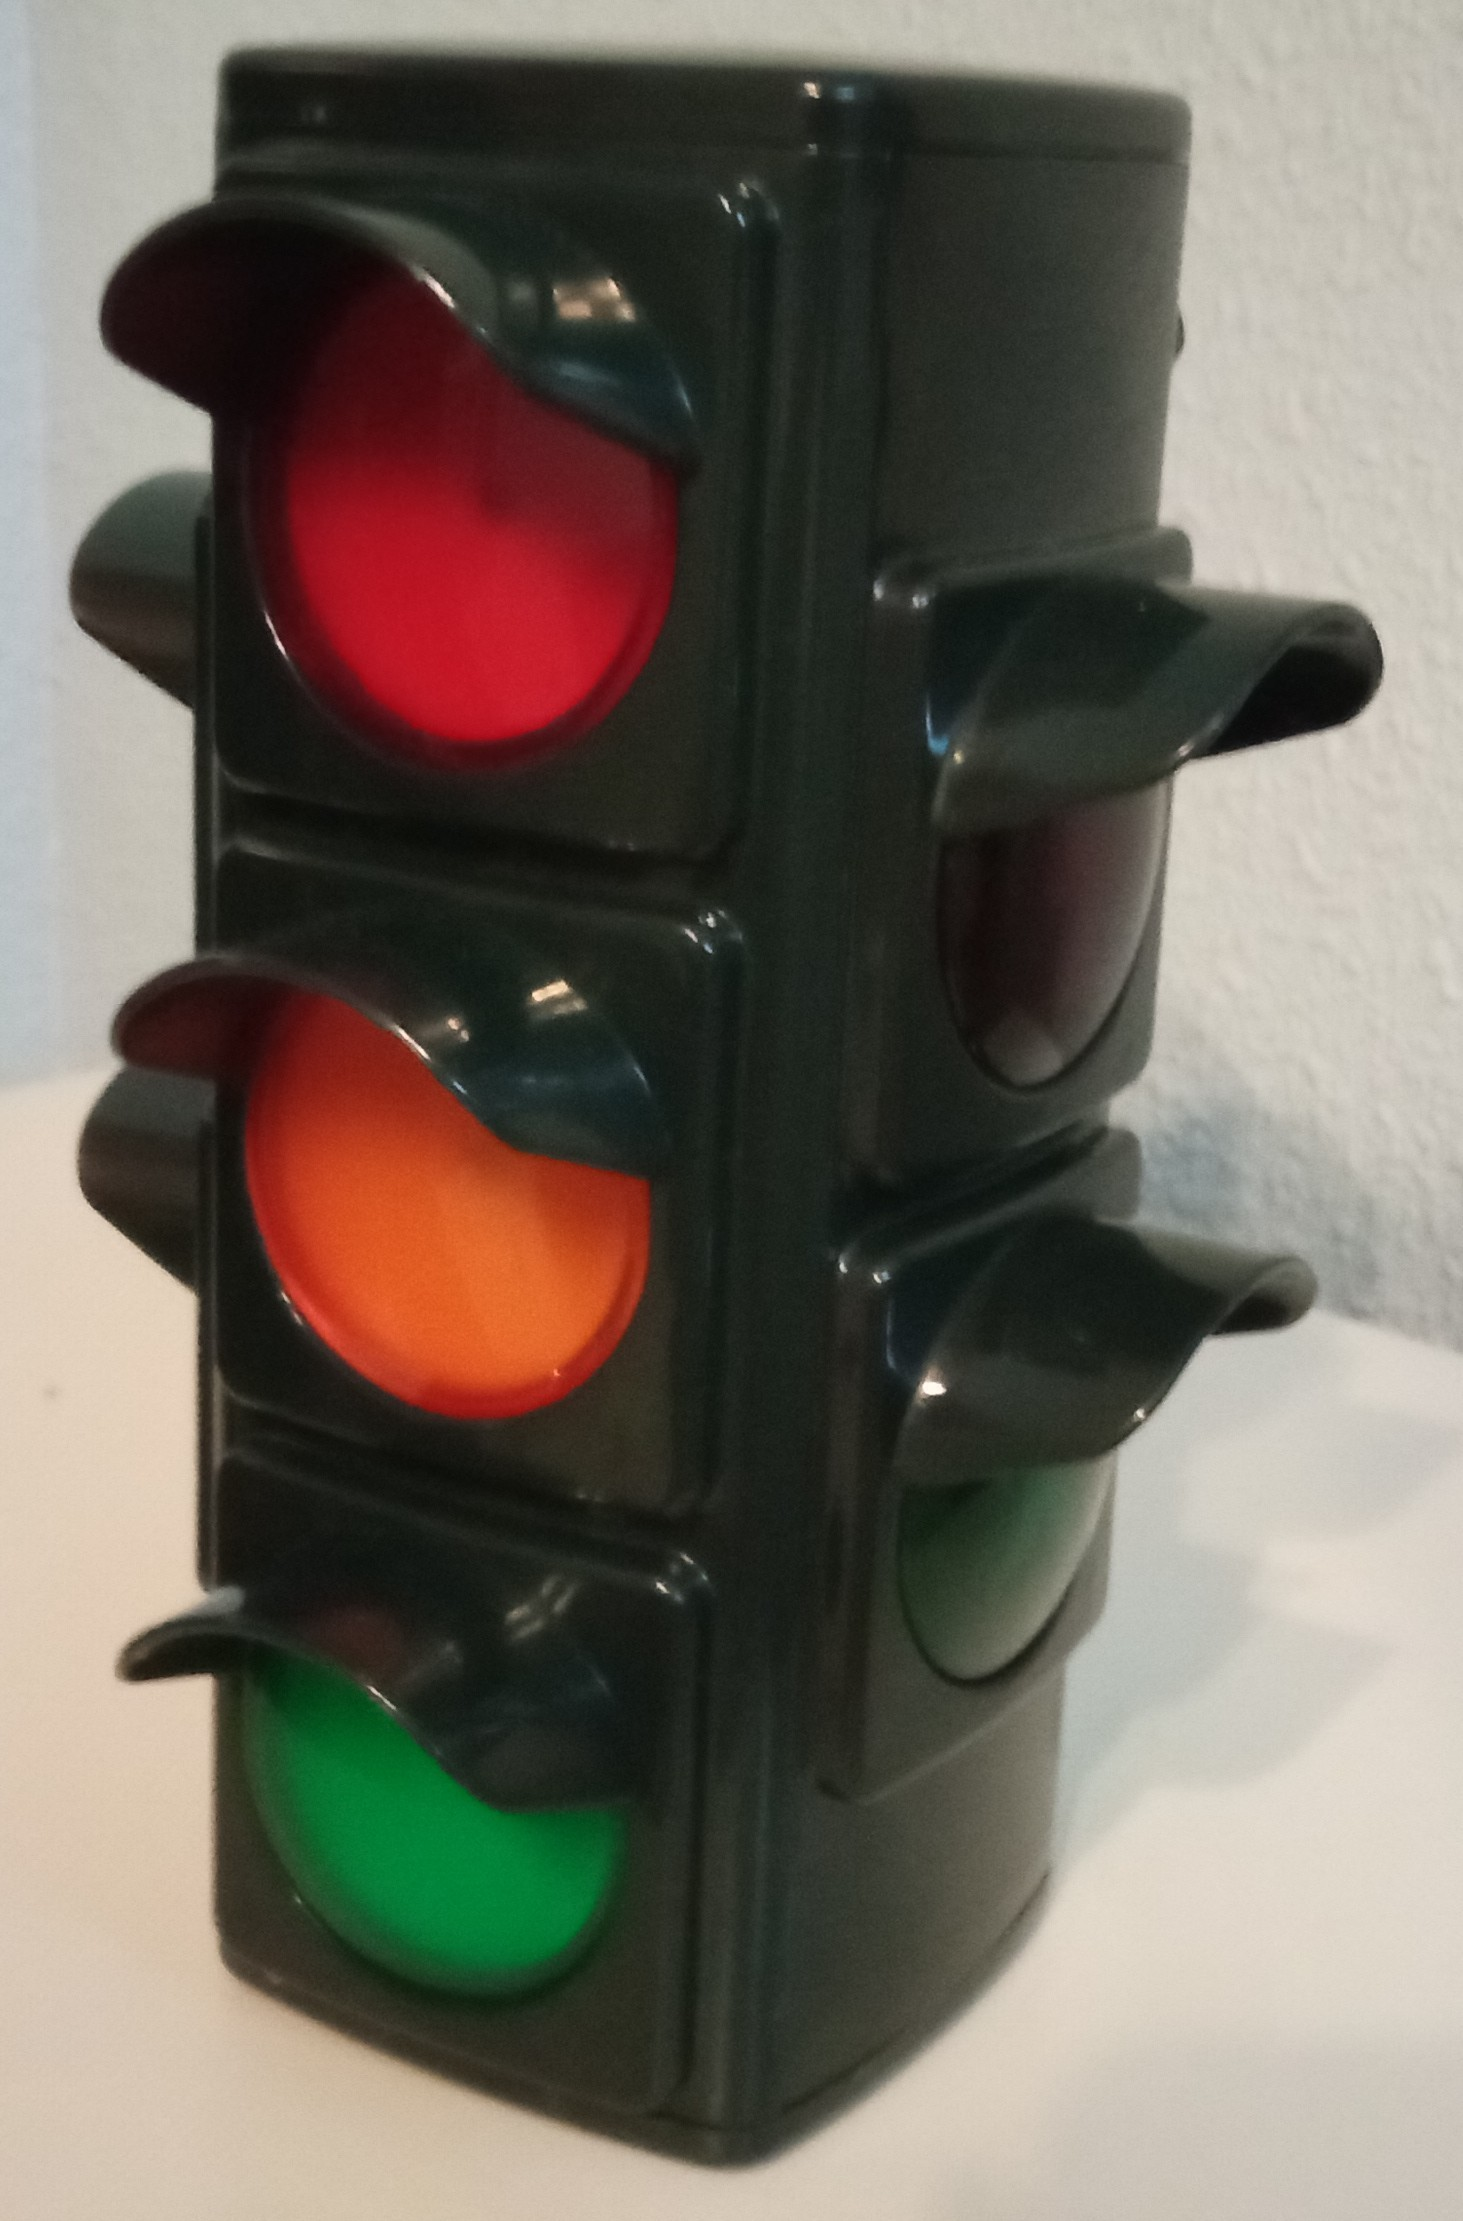
\includegraphics[width=2cm,
			height=2.5cm]{figs/realtrafficlight}\hspace{0.7cm}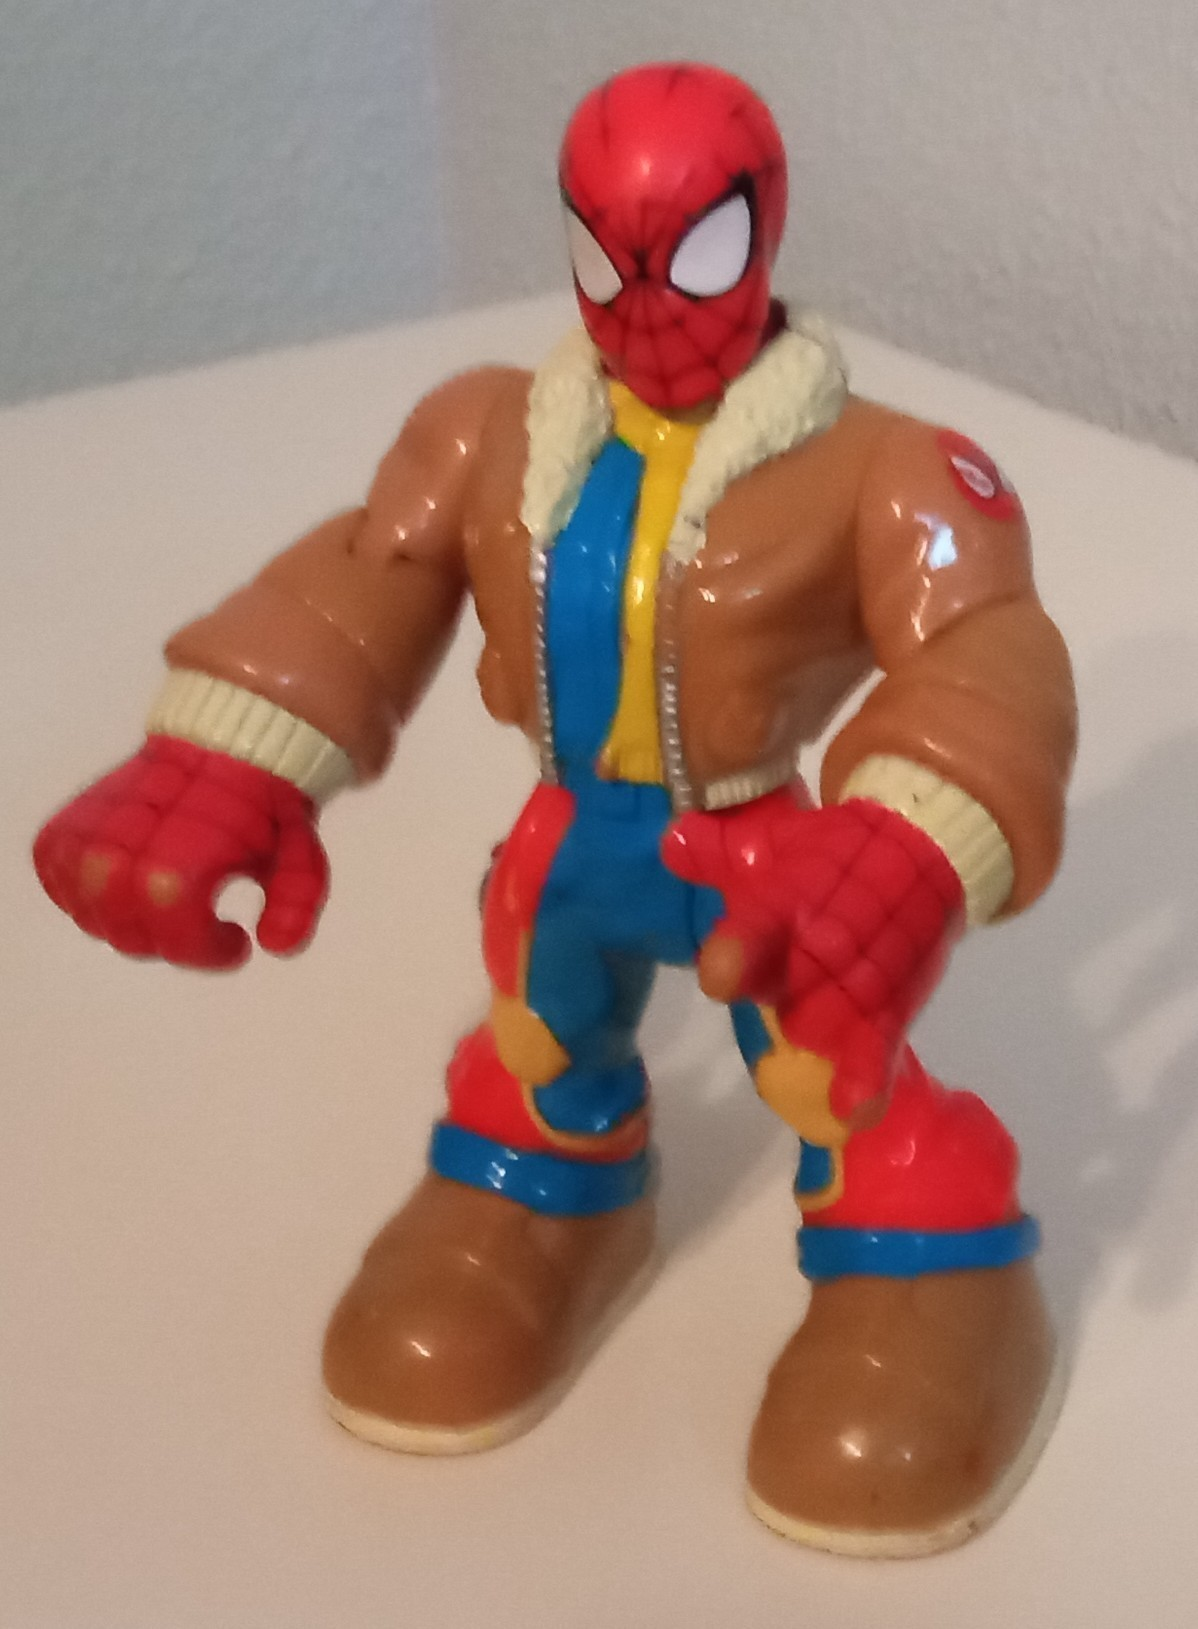
\includegraphics[width=2cm, height=2.5cm]{figs/realpedestrian}
	\end{figure}
	\note[item]{Entorno real.}
\end{frame}

\begin{frame}
	\frametitle{Circuito inicial}
	\begin{figure}
		\centering
		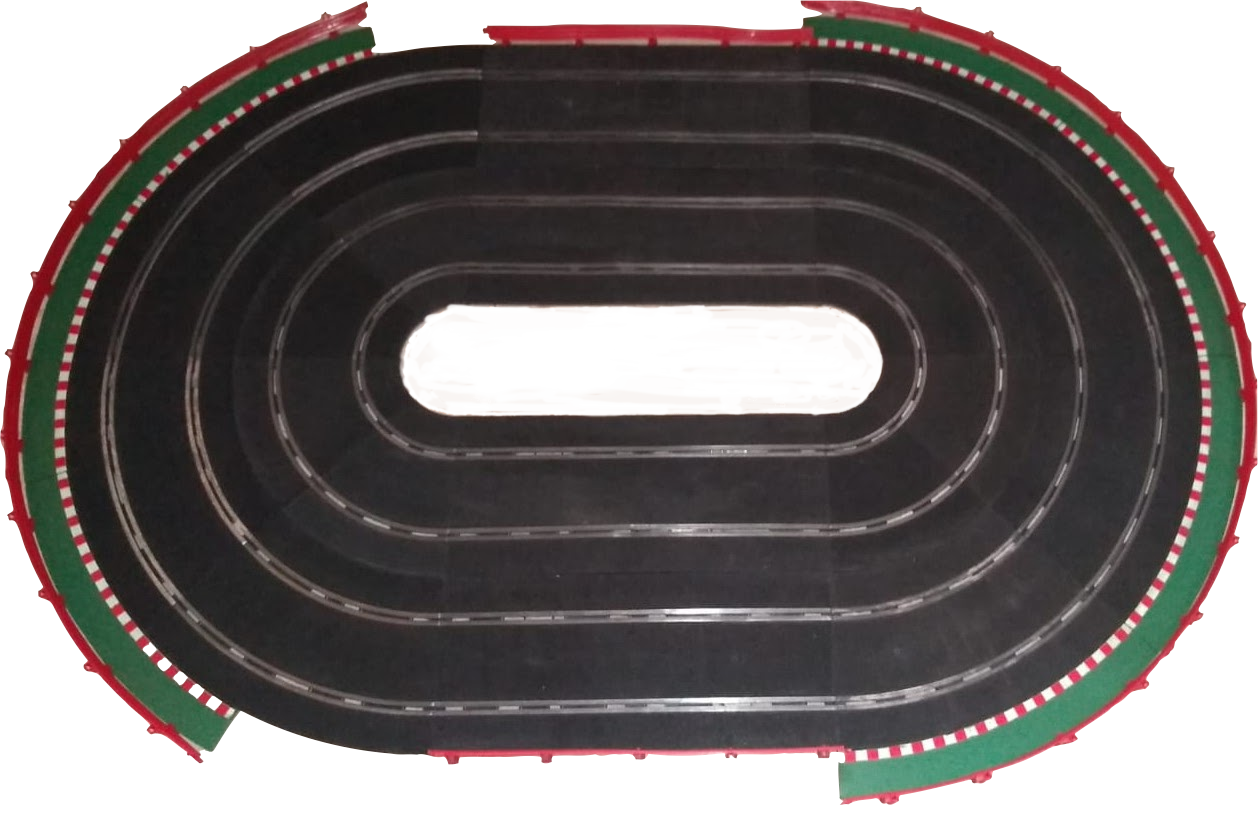
\includegraphics[width=6cm]{figs/circuit}
	\end{figure}
	\begin{outline}
		\1 Entrenamiento con luz \textcolor{red}{\textit{artificial}}.
	\end{outline}
	\note[item]{Circuito incial.}
\end{frame}

\begin{frame}
	\frametitle{Circuito con objetos}
	\begin{figure}
		\centering
		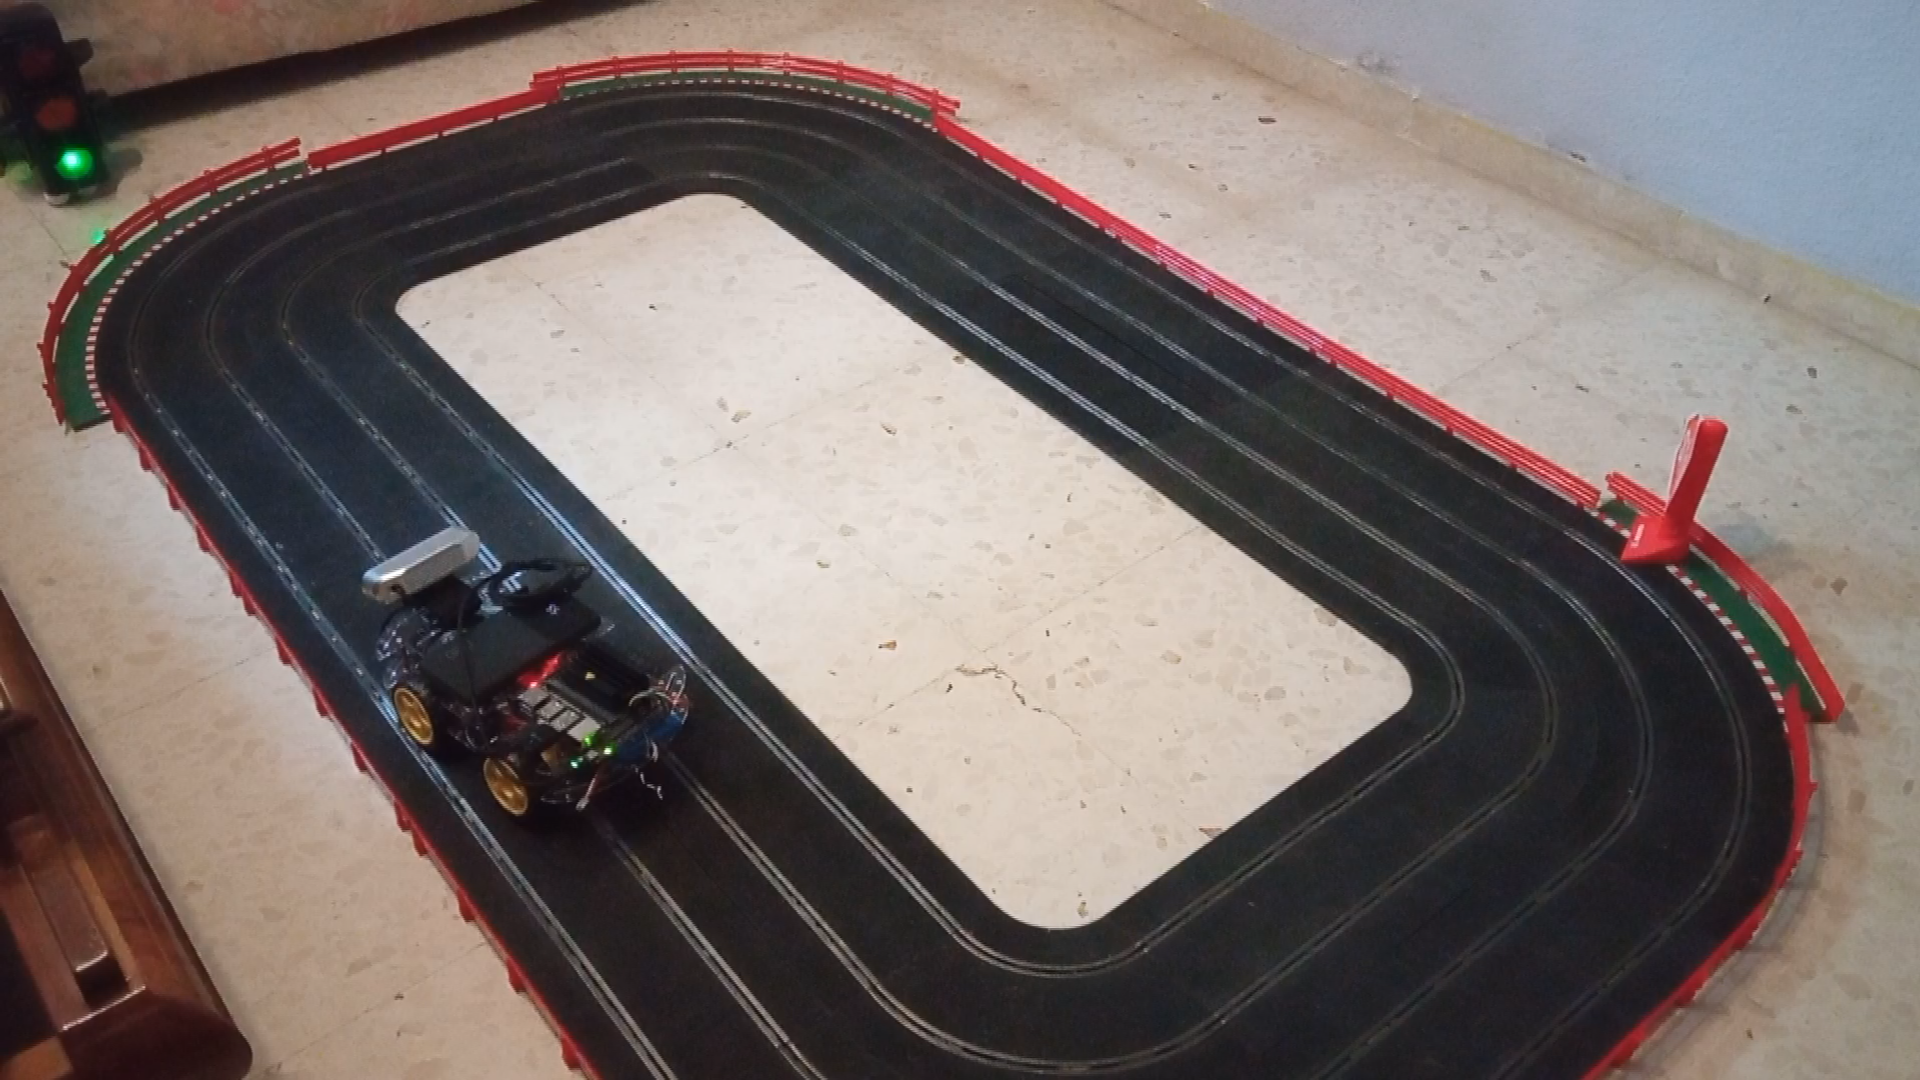
\includegraphics[width=10cm]{figs/circuitwithobjects2}
	\end{figure}
	\note[item]{Circuito con objetos.}
\end{frame}

\begin{frame}
	\frametitle{\textit{Dataset} objetos reales}
	\begin{figure}
		\centering
		\includegraphics[height=3cm]{figs/datasetone}\hspace{0.5cm}
		\includegraphics[width=4cm]{figs/datasettwo}\hspace{0.5cm}\\
		\vspace{1cm}\includegraphics[width=4cm]{figs/datasetthree}\hspace{0.5cm}
		\includegraphics[width=4cm]{figs/datasetfour}
	\end{figure}
	\note[item]{Dataset objetos reales.}
\end{frame}

\begin{frame}
	\frametitle{Entrenamiento red de detección de objetos}
	\begin{figure}
		\centering
		\includegraphics[width=10cm]{figs/fan}
	\end{figure}
	\begin{outline}
		\1 Portátil con \textcolor{red}{\textit{NVIDIA MX330}} $\simeq 95^\circ C$.
		\1 2000 iteraciones $\simeq$ 3 horas.
		\1 Únicamente con \textcolor{red}{\textit{dataset}} propio.
	\end{outline}
	\note[item]{Entrenamiento red de detección de objetos.}
\end{frame}

\begin{frame}
	\frametitle{Entrenamiento red de detección de objetos}
	\begin{figure}
		\centering
		\includegraphics[width=7cm]{figs/chart}
	\end{figure}
	\note[item]{Entrenamiento red de detección de objetos.}
\end{frame}

\begin{frame}
	\frametitle{Comparación probabilidad de detección}
	\begin{outline}
		\1 Imagen nueva para ambas redes.
	\end{outline}
	\begin{figure}
		\centering
		\includegraphics[width=5.8cm]{figs/predictionsoriginal}\hspace{0.1cm}
		\includegraphics[width=5.8cm]{figs/predictionscustom}
	\end{figure}
	\note[item]{Comparación probabilidad de detección.}
	\note[item]{Marca la diferencia entre detectar o no al peatón cuando el robot está en movimiento.}
\end{frame}

\begin{frame}
	\frametitle{Ejecución en el entorno real}
	\begin{figure}
		\centering
		\includegraphics[width=3.5cm, height=3.5cm]{figs/screenshottrafficlight}\\\vspace{0.5cm}
		\includegraphics[width=3.5cm,
			height=3.5cm]{figs/screenshotstopsign}\hspace{1cm}\includegraphics[width=3.5cm, height=3.5cm]{figs/screenshotpedestrian}
	\end{figure}
	\note[item]{Ejecución en el entorno real.}
\end{frame}

% \begin{conditions*}
% 	R & resistencia del material $[\Omega]$\\
% 	\rho & resistividad $[\Omega-m]$\\
% 	l & longitud $[m]$\\
% 	A & área de sección transversal $[m^2]$
% \end{conditions*}

%%%%%%%%%%%%%%%%%%%%%%%%%%%%%%%%%%%%%%%%%%%%%%%%%%%%%%%% Capítulo 5 %%%%%%%%%%%%%%%%%%%%%%%%%%%%%%%%%%%%%%%%%%%%%%%%%%%%%%%%%%%%%% 

\section*{}
\begin{frame}{}
	\centering \Huge
	\emph{Conclusiones}
	\note[item]{Para acabar esta presentación, vamos a repasar lo hecho, unas breves conclusiones y las líneas futuras.}
\end{frame}

\section{Conclusiones}
\begin{frame}
	\frametitle{Conclusiones}
	\begin{outline}
		\1 Para lograr los objetivos se han utilizado dos \textcolor{red}{redes neuronales}:
		\2 Seguimiento de carril: librería \textcolor{red}{\textit{JetRacer}} que implementa una red \textcolor{red}{\textit{residual}} \textit{ResNet-18} combinada con un
		\textcolor{red}{controlador}.
		\2 Detección de objetos: \textit{framework} \textcolor{red}{\textit{Darknet}} que permite ejecutar una red \textcolor{red}{\textit{convolucional}} \textit{YOLO V3
			Tiny} previamente entrenada mediante un \textcolor{red}{\textit{dataset}} propio con los objetos reales para aumentar la fiabilidad.
		\1 Todo ello ha sido combinado en dos paquetes \textcolor{red}{\textit{ROS}}, diferenciando entorno simulado y real.
		\1 Limitaciones: \textcolor{red}{ángulo} de la cámara y \textcolor{red}{resolución} de imagen en las redes neuronales.
	\end{outline}
	\note[item]{Conclusiones.}
\end{frame}

\subsection{Líneas futuras}
\begin{frame}
	\frametitle{Líneas futuras}
	\begin{figure}
		\centering
		\includegraphics[width=5cm]{figs/tunel}\hspace{0.5cm}
		\includegraphics[width=5cm]{figs/forest}
	\end{figure}
	\note[item]{Líneas futuras: mayor dataset, túnes, bosques, todo entorno donde exista algo similar a un camino a seguir. También sería interesante obtener los límites en
		izquierda y derecha del carril y no solo el punto central.}
\end{frame}

\begin{frame}[plain]
	\large{\titlepage}
	\note[item]{Vídeo.}
	\note[item]{Eso sería todo. Muchas gracias por su atención.}
\end{frame}

\end{document}